\documentclass[a4paper, 12pt]{article}

\usepackage{hyperref}
\usepackage[warn]{mathtext}
\usepackage[utf8]{inputenc}
\usepackage[T2A]{fontenc}
\usepackage[english,russian]{babel}
\usepackage{multirow}
\usepackage{amsmath,amsfonts,amssymb,amsthm,mathtools}
\usepackage{indentfirst}
\DeclareSymbolFont{T2Aletters}{T2A}{cmr}{m}{it}
\usepackage{ gensymb }
\mathtoolsset{showonlyrefs=true}
\usepackage{euscript}
\usepackage{mathrsfs}
\usepackage[left=2cm,right=2cm,top=2cm,bottom=2cm]{geometry}
\usepackage{graphicx}
\usepackage{wrapfig}
\usepackage[rgb]{xcolor}
\hypersetup{
colorlinks=true,
urlcolor=blue
}


\title{Лабораторная работа 1.3.3}
\author{Гисич Арсений Б03-109}
\date{2022}

\begin{document}

	\begin{center}
		{\large МОСКОВСКИЙ ФИЗИКО-ТЕХНИЧЕСКИЙ ИНСТИТУТ (НАЦИОНАЛЬНЫЙ ИССЛЕДОВАТЕЛЬСКИЙ УНИВЕРСИТЕТ)}
	\end{center}
	\vspace{5 cm}
	{\Large
		\begin{center}
			{\bf Лабораторная работа 1.3.3}\\[0.2 cm]
			Измерение вязкости воздуха по течению в тонких трубках
		\end{center}
	}
	\vspace{4 cm}
	\begin{flushright}
		{\Large Выполнил: \\
			\vspace{0.2 cm}
			Гисич Арсений \\
			\vspace{0.2 cm}
			Б03-109 \\}
	\end{flushright}
	\vspace{9 cm}
	\begin{center}
		Долгопрудный\\[0.1 cm]
		2022
	\end{center}
\thispagestyle{empty}

\section{Аннотация}

\par Цель работы: экспериментально исследовать свойства течения газов по тонким трубкам при различных числах Рейнольдса; выявить область применимости закона Пуазейля и с его помощью определить коэффициент вязкости воздуха.

\section{Теоретические сведения}

\par Работа посвящена изучению течения воздуха по прямой трубе круглого сечения. Движение жидкости или газа вызывается перепадом внешнего давления на концах $\Delta{P}$ трубы, чему в свою очередь препятствуют силы вязкого
(«внутреннего») трения, действующие между соседними слоями жидкости, а
также со стороны стенок трубы.
\par Сила вязкого трения как в жидкостях, так и в газах описывается законом
Ньютона: касательное напряжение между слоями пропорционально перепаду
скорости течения в направлении, поперечном к потоку. В частности, если жидкость течёт вдоль оси $x$, а скорость течения $v_x(y)$ зависит от координаты $y$, в каждом слое возникает направленное по $x$ касательное напряжение 
\begin{equation}\label{1}
\tau_{xy} = -\eta\frac{\delta{v_x}}{\delta_y}.
\end{equation}
Величину $\eta$ называют коэффициентом динамической вязкости (или просто
вязкостью) среды.
\par Объёмным расходом (или просто расходом) $Q$ называют объём жидкости,
протекающий через сечение трубы в единицу времени. Величина $Q$ зависит от
перепада давления $\Delta{P}$, а также от свойств газа (плотности $\rho$ и вязкости $\eta$) и от
геометрических размеров (радиуса трубы $R$ и её длины $L$). Основная задача
данной работы — исследовать эту зависимость экспериментально.
\par Характер течения в трубе может быть ламинарным либо турбулентным.
При ламинарном течении поле скоростей $u(r)$ образует набор непрерывных
линий тока, а слои жидкости не перемешиваются между собой. Турбулентное течение характеризуется образованием вихрей и активным перемешиванием
слоев, при этом даже в стационарном течении в каждой точке имеют место
существенные флуктуации скорости течения и давления.
\par Характер течения определяется безразмерным параметром задачи — числом Рейнольдса:
\begin{equation}\label{2}
Re = \frac{\rho{ua}}{\eta}.
\end{equation}
где $\rho$ — плотность среды, $u$ — характерная скорость потока, $\eta$ — коэффициент вязкости среды, $a$ — характерный размер системы (размер, на котором
существенно меняется скорость течения). Это число имеет смысл отношения
кинетической энергии движения элемента объёма жидкости к потерям энергии из-за трения в нём $Re \sim K/A_{\text{тр}}$. При достаточно малых $Re$ в потоке доминируют вязкие силы трения и течение, как правило, является ламинарным.
С ростом числа Рейнольдса может быть достигнуто его критическое значение $Re_{\text{кр}}$, при котором характер течения сменяется с ламинарного на турбулентный.
\par Из опыта известно, что переход к турбулентному течению по трубкам
круглого сечения наблюдается при $Re_{\text{кр}} \approx 10^3$ (здесь в качестве $u$ выбрана средняя скорость потока, определяемая через полный расход $Q$ как $\overline{u}=\frac{Q}{\pi{R^2}}$, а в качестве характерного размера — радиус трубы $R$). Стоит отметить, что значение $Re_{\text{кр}}$ не является универсальным и зависит от геометрии задачи: например, при обтекании сферических или цилиндрических тел потоком жидкости
оно составляет всего несколько десятков ($Re_{\text{кр}} \sim 10 \div 20$).
\par В целях упрощения теоретической модели течение газа в условиях эксперимента можно считать несжимаемым, то есть принять плотность среды постоянной: $\rho = const$. Для газов такое приближение допустимо, если относительный перепад давления в трубе мал $\Delta{P} \ll P$, а скорость течения значительно меньше скорости звука (число Маха много меньше единицы). В нашем
опыте максимальная разность давлений составляет $\sim 30~\text{см}$ водного столба
(3 кПа), что составляет $\sim 3\%$ от атмосферного давления, причем в «рабочем»
(ламинарном) режиме перепад в несколько раз меньше ($\sim 5 \div 10~\text{см вод. ст.}$).
\par {\bf Течение Пуазейля.} Из опыта известно, что при достаточно малых числах
Рейнольдса течение в прямой трубе с гладкими стенками имеет ламинарный
характер. В таком случае задача о течении жидкости имеет простое аналитическое решение.
\par Направим ось $x$ вдоль трубы по направлению потока. В ламинарном потоке
скорость течения среды $u$ будет направлена всюду по $x$ (линии тока параллельны стенкам трубки), а давление постоянно в пределах любого сечения и зависит только от продольной координаты $P(x)$. Будем искать частное решение — установившееся течение, в котором профиль скорости $u(r)$ (распределение скорости в зависимости от расстояния до оси $r$) одинаков в любом поперечном сечении, то есть не зависит от $x$.
\begin{wrapfigure}{|}{6cm}
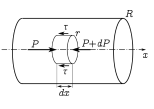
\includegraphics[scale=1.2]{1.png}
\caption{К выводу формулы Пуазейля}
\label{ris1}
\end{wrapfigure}
\par Выделим соосный трубе цилиндр некоторого радиуса $r$ и длины $dx$ (см.
Рис. \ref{ris1}). Поскольку при стационарном течении жидкость течёт без ускорения,
сумма всех сил, действующих на жидкость в цилиндре, должна быть равна
нулю. На жидкость внутри цилиндра действует направленная вдоль оси трубы
сила $F_{1x} = -dP \cdot \pi{r^2},$
где $dP = P(x + dx) - P(x) < 0$ — разность давлений в сечениях на торцах
выделенного участка. На боковые поверхности цилиндра действует касательная сила вязкого трения
\begin{equation}\label{3}
F_{2x} = -\tau \cdot 2\pi{rdx},
\end{equation}
где согласно закону Ньютона \eqref{1} касательное напряжение равно
\begin{equation}\label{4}
\tau = -\eta\frac{du}{dr}.
\end{equation}
Из условия баланса сил $F_{1x} + F_{2x} = 0$ находим
\begin{equation}\label{5}
\frac{dP}{dx} = -\eta\frac{2du}{rdr}.
\end{equation}
В установившемся течении правая часть полученного выражения является
функцией только радиуса $r$. В левой части \eqref{5} находится градиент давления,
который не зависит от $r$ вовсе, и, следовательно, обе части уравнения \eqref{5} являются константами. Тогда, проводя интегрирование, приходим к следующему. Во-первых, давление в трубе является линейно убывающей функцией
координаты
\begin{equation}\label{6}
P(x) = P_0 - \frac{\Delta{P}}{l}x,
\end{equation}
где $\Delta{P}$ — перепад давления на участке длиной $l$, $P_0$ — давление в начале
участка (в точке $x = 0$). Во-вторых, профиль скорости является параболической функцией с максимумом на оси трубы
\begin{equation}\label{7}
u(r) = u_{max} - \frac{\Delta{P}}{4l}r^2.
\end{equation}
Для нахождения константы интегрирования $u_{max}$ необходимо дополнительно задать граничное условие. Для течения вязкой жидкости обычно используют так называемое условием прилипания: касательная скорость потока вблизи стенок считается равной скорости движения самих стенок. Физически
это означает, что на молекулярном уровне стенки являются шероховатыми,
так что при ударе о них молекулы в среднем полностью теряют направленную
$x$-компоненту импульса. В рассматриваемой задаче стенки неподвижны, поэтому имеем
\begin{equation}\label{8}
u|_{r=R} = 0.
\end{equation}
Отсюда находим $u_{max} = \frac{\Delta{P}}{4L}R^2$ и профиль скорости
\begin{equation}\label{9}
u(r) = \frac{\Delta{P}}{4L}(R^2 - r^2).
\end{equation}
Наконец, интегрируя $u(r)$ по сечению трубы, получим объёмный расход жидкости в зависимости от перепада давления на концах:
\begin{equation}\label{10}
Q = \int_0^R u(r) \cdot 2\pi rdr=\frac{\pi R^4\Delta{P}}{8\eta l}.
\end{equation}
Это соотношение называют формулой Пуазейля. Заметим, что средняя скорость потока при пуазейлевском течении, как видно из \eqref{10}, оказывается
вдвое меньше максимальной:
\begin{equation}\label{11}
\overline{u} \equiv \frac{Q}{\pi R^2} = \frac{u_{max}}{2}.
\end{equation}
\par Формула Пуазейля \eqref{10} позволяет найти вязкость газа по зависимости расхода от перепада давления в трубе и используется в качестве основной расчётной формулы в данной работе.
\par {\bf Длина установления.} Пусть на вход трубы поступает течение, распределение скоростей которого не является пуазейлевским (например, распределение скоростей равномерное, как на Рис. \ref{ris3}). Ясно, что профиль течения \eqref{9} не может установиться сразу, а реализуется лишь на некотором расстоянии $l_{\text{уст}}$ от начала трубы. Оценим эту длину по порядку величины.
\begin{wrapfigure}{r}{0.3\textwidth}
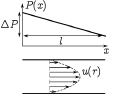
\includegraphics[width=0.25\textwidth]{2.png}
\caption{Распределение давления и скорости течения Пуазейля в трубе}
\label{ris2}
\end{wrapfigure}
\par Рассмотрим слой жидкости толщиной $dx$ в поперечном сечении трубы. Кинетическая энергия, запасённая в нём, составляет
\begin{wrapfigure}{|}{0.5\textwidth}
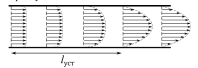
\includegraphics[width=0.3\textwidth]{3.png}
\caption{Формирование установившегося течения (в ламинарном режиме)}
\label{ris3}
\end{wrapfigure}
\begin{equation}\label{12}
K \sim \frac{1}{2}\rho u^2 \cdot \pi R^2dx.
\end{equation}
Работу, которую совершат вязкие силы трения по перемещению этого слоя на
расстояние $l$, можно оценить как
\begin{equation}\label{13}
A_{\text{тр}} \sim \eta\frac{du}{dr} \cdot \pi R^2dx \cdot l.
\end{equation}
Для перепада скоростей воспользуемся оценкой $\frac{du}{dr} \sim \frac{\Delta{u}}{R} \sim \frac{u}{R}$. Наконец, примем, что работа сил трения, необходимая для перераспределения скоростей,
по порядку величины равна кинетической энергии $K \sim A_{\text{тр}}$. Тогда, отбрасываячисленные коэффициенты порядка единицы, получаем грубую оценку для
длины установления:
\begin{equation}\label{14}
l_{\text{уст}} \sim \frac{\rho u R^2}{\eta} = R \cdot Re.
\end{equation}
Точный численный коэффициент здесь аналитически установить затруднительно (к тому же, он зависит от вида начального распределения $u(r)$. Как
показывает опыт, этот коэффициент можно с удовлетворительной точностью
принять равным 0,2:
\begin{equation}\label{15}
l_{\text{уст}} \equiv 0,2R \cdot Re.
\end{equation}
Заметим, что если длина трубы мала по сравнению с $l_{\text{уст}}$, то работой сил трения в ней можно пренебречь и течение в ней будет описываться не формулой
Пуазейля, а уравнением Бернулли (при условии, что течение останется ламинарным).
\par Экспериментально длину установления можно определить, измеряя распределение давления вдоль трубки $P(x)$. На неустановившемся участке будет
наблюдаться отклонение от линейного закона \eqref{6}, и при том же расходе $Q$ градиент давления $ \frac{\Delta{P}}{l} $ будет больше, чем следует из формулы Пуазейля.
\par {\bf Вязкость газов.} Рассмотрим механизм возникновения вязкости в газах.
Молекулы газа участвуют как в направленном движении со средней скоростью потока $u$, так и в хаотическом тепловом движении, характеризующимся средней тепловой скоростью $ \overline{v} = \sqrt{\frac{8k_{\text{Б}}T}{\pi m}}$ (здесь $m$ — масса молекулы). Молекулы могут свободно перемещаться между слоями и обмениваться друг с другом импульсами при столкновениях. Если в двух соседних слоях потоковые
скорости различны, то такой обмен импульсом и приводит к эффективному
возникновению силы трения между слоями.
\par Исходя из приведенных соображений можно получить следующую
оценку для коэффициента вязкости идеального газа:
\begin{equation}\label{16}
\eta \sim \frac{1}{3}\rho \overline{v} \lambda,
\end{equation}
где $\lambda$ — длина свободного пробега молекул газа относительно столкновений
друг с другом. Как известно из молекулярно-кинетической теории, длина пробега определяется эффективным («газокинетическим») диаметром молекул $d$
как $\lambda \sim 1/(n\pi d^2)$, где $n$ — объёмная концентрация газа. Видно, что $\lambda$ обратно пропорциональна плотности газа, поэтому, как следует из \eqref{16}, вязкость газа не зависит от его плотности и определяется только температурой $T$. Данный вывод может показаться парадоксальным, поскольку в более плотном газе большее число молекул должно участвовать в передаче импульса между слоями, однако это компенсируется тем, что этот импульс передается на меньшее
расстояние.
\par Заметим также, что закон Ньютона \eqref{1} и формула \eqref{16} для газов применимы, только когда скорость потока мала по сравнению с тепловой $u \ll \overline{v}$ , а характерные размеры системы значительно превышают длину свободного пробега молекул (т.е. система не находится в состоянии высокого вакуума).
\section{Методика измерений}

\par Схема экспериментальной установки изображена на Рис. \ref{ris4}. Поток воздуха
под давлением, немного превышающим атмосферное, поступает через газовый счётчик в тонкие металлические трубки. Воздух нагнетается компрессором, интенсивность его подачи регулируется краном К. Трубки снабжены съёмными заглушками на концах и рядом миллиметровых отверстий, к которым можно подключать микроманометр. В рабочем состоянии открыта заглушка на одной (рабочей) трубке, микроманометр подключён к двум её выводам, а все остальные отверстия плотно закрыты пробками.
Перед входом в газовый счётчик установлен водяной U-образный манометр. Он служит для измерения давления газа на входе, а также предохраняет счётчик от выхода из строя. При превышении максимального избыточного давления на входе счётчика ($\sim  30~\text{см вод. ст.}$) вода выплёскивается из трубки в защитный баллон Б, создавая шум и привлекая к себе внимание экспериментатора.
\begin{figure}[h!]
\begin{center}
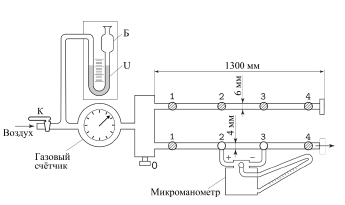
\includegraphics[scale=1.2]{4.png}
\caption{Экспериментальная установка}
\label{ris4}
\end{center}
\end{figure}
\par {\bf Газовый счётчик.} В работе используется газовый счётчик барабанного
типа, позволяющий измерять объём газа $\Delta{V}$, прошедшего через систему. Измеряя время $\Delta{t}$ при помощи секундомера, можно вычислить средний объёмный расход газа $Q=\Delta{V}/\Delta{t}$ (для получения массового расхода [кг/с] результат необходимо домножить на плотность газа $\rho$).
\begin{wrapfigure}{r}{0.4\textwidth}
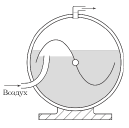
\includegraphics[width=0.25\textwidth]{5.png}
\caption{Принцип работы барабанного газосчётчика}
\label{ris5}
\end{wrapfigure}
\par Работа счётчика основана на принципе вытеснения: на цилиндрической ёмкости жёстко укреплены лёгкие чаши (см. Рис. \ref{ris5}, где для
упрощения изображены только две чаши), в которые поочередно поступает воздух из входной трубки расходомера. Когда чаша наполняется, она всплывает и её место занимает следующая и т.д. Вращение оси предаётся на счётно-суммирующее устройство.
\par Для корректной работы счётчика он должен быть заполнен водой и установлен горизонтально по уровню (подробнее см. техническое описание установки).
\par {\bf Микроманометр.} В работе используется жидкостный манометр с наклонной трубкой. Разность давлений на входах манометра измеряется по высоте
подъёма рабочей жидкости (как правило, этиловый спирт). Регулировка
наклона позволяет измерять давление в различных диапазонах.
\par На крышке прибора установлен трехходовой кран, имеющий два рабочих
положения — (0) и (+). В положении (0) производится установка мениска жидкости на ноль, что необходимо сделать перед началом работы (в процессе работы также рекомендуется периодически проверять положение нуля). В положении (+) производятся измерения.
\par При работе с жидкостным манометром важно не допустить его «зашкаливания» — перелива рабочей жидкости в подводящие трубки (в этом случае
работу придется приостановить для просушки трубок, долива спирта и т.д.).
Все манипуляции по перестановке измерительных трубок следует проводить,
когда манометр находится в положении (0). Подачу газа в систему, наоборот,
следует осуществлять в положении (+), чтобы контролировать величину давления и иметь возможность вовремя перекрыть поток.
\par Перед началом работы с микроманометром необходимо убедиться, что в
нём залито достаточное количество спирта, а сам манометр установлен строго
горизонтально по уровням. Подводящие трубки, заполненные спиртом, не
должны содержать пузырьков воздуха, а в трубках, заполненных воздухом, не
должно быть капель спирта. Подробнее инструкцию по подготовке прибора к
работе см. в техническом описании установки.
\section{Используемое оборудование}

\begin{enumerate}
    \item Система подачи воздуха (компрессор, проводящие трубки);
    \item Газовый счётчик барабанного типа,  $\delta_{\text{счётчика}} = 0,01~\text{л}$;
    \item Спиртовой микроманометр с регулируемым наклоном,  $\delta_{\text{мкманом}} = 0,05~\text{см}$;
    \item U-образный манометр,  $\delta_{\text{маном}} = 0,25~\text{см}$;
    \item Набор трубок различного диаметра с выходами для подсоединения микроманометра;
    \item Секундомер;
\end{enumerate}

\section{Результаты измерений и обработка данных}

Начальные условия:\par

$\begin{aligned}
& P_{\text{атм}} = 98,40\pm0,05~\text{кПа}\\
& T = 23,8\pm0,1~\celsius
\end{aligned}$\\[0,5 cm]
\subsection{1 трубка}
\par Проведём предварительные расчёты для первой трубки ($l = 0,9~\text{м}, d_1 = 5,25\pm0,05~\text{мм}$). $Q_{\text{кр}} = \overline{u}\pi r^2 = \frac{Re_{\text{кр}}\eta\pi R}{\rho}$. Из закона Менделеева-Клапейрона $\rho = \frac{P_{\text{атм}}\mu}{RT}$. Тогда
\begin{equation}\label{17}
Q_{\text{кр}} = \frac{Re_{\text{кр}}\eta\pi rRT}{P_{\text{атм}}\mu}.
\end{equation}
При $Re_{\text{кр}} \approx 10^3, \eta \sim 2\cdot 10^{-5}$ Па $\cdot$ с получаем $Q_{\text{кр}} \approx 14,3 \cdot 10^{-5}$ м$^3$/с.
\par По формуле Пуазейля \eqref{10} находим
\begin{equation}\label{18}
\Delta{P} = \frac{Q_{\text{кр}}8\eta l}{\pi r^4}.
\end{equation}
Полученное значение $\Delta{P} \approx 138~\text{Па}$, т. е. 70 делений микроманометра.
\par По формуле \eqref{15} оценим длину $l_{\text{уст}} \approx 0,53~\text{м}$, что меньше длины выбранного участка. Значит, течение можно считать установившимся.

\par Полученные результаты измерения $\Delta{P}(Q)$ при ламинарном течении представленны в таблице \ref{tab1}.
\begin{table}[h!]
\begin{tabular}{|c|c|c|c|c|c|c|c|c|c|}
\hline
$\Delta{P}$, дел    & $\Delta{P}$, Па           & $\delta_{\Delta{P}}$, Па  & $\Delta{t}$, с & $\overline{\Delta{t}}$, c & $\delta_{\overline{\Delta{t}}}$, с & $\Delta{V}$, л     & $\delta_{\Delta{V}}$, л & $Q$, м$^3$/c      & $\delta_{Q}$, м$^3$/с \\ \hline
\multirow{5}{*}{25} & \multirow{5}{*}{49,03325} & \multirow{5}{*}{0,980665} & 22,16          & \multirow{5}{*}{23,16}    & \multirow{5}{*}{0,65908}           & \multirow{5}{*}{1} & \multirow{5}{*}{0,01}   & \multirow{5}{*}{0,0000432} & \multirow{5}{*}{0,0000013}    \\ \cline{4-4}
                    &                           &                           & 21,30          &                           &                                    &                    &                         &                            &                               \\ \cline{4-4}
                    &                           &                           & 23,20          &                           &                                    &                    &                         &                            &                               \\ \cline{4-4}
                    &                           &                           & 24,45          &                           &                                    &                    &                         &                            &                               \\ \cline{4-4}
                    &                           &                           & 24,71          &                           &                                    &                    &                         &                            &                               \\ \hline
\multirow{5}{*}{32} & \multirow{5}{*}{62,76256} & \multirow{5}{*}{0,980665} & 15,13          & \multirow{5}{*}{14,85}    & \multirow{5}{*}{0,3647}            & \multirow{5}{*}{1} & \multirow{5}{*}{0,01}   & \multirow{5}{*}{0,0000674} & \multirow{5}{*}{0,0000018}    \\ \cline{4-4}
                    &                           &                           & 15,73          &                           &                                    &                    &                         &                            &                               \\ \cline{4-4}
                    &                           &                           & 15,33          &                           &                                    &                    &                         &                            &                               \\ \cline{4-4}
                    &                           &                           & 14,16          &                           &                                    &                    &                         &                            &                               \\ \cline{4-4}
                    &                           &                           & 13,88          &                           &                                    &                    &                         &                            &                               \\ \hline
\multirow{5}{*}{38} & \multirow{5}{*}{74,53054} & \multirow{5}{*}{0,980665} & 12,01          & \multirow{5}{*}{12,80}    & \multirow{5}{*}{0,2449}            & \multirow{5}{*}{1} & \multirow{5}{*}{0,01}   & \multirow{5}{*}{0,0000781} & \multirow{5}{*}{0,0000017}    \\ \cline{4-4}
                    &                           &                           & 12,76          &                           &                                    &                    &                         &                            &                               \\ \cline{4-4}
                    &                           &                           & 13,23          &                           &                                    &                    &                         &                            &                               \\ \cline{4-4}
                    &                           &                           & 13,27          &                           &                                    &                    &                         &                            &                               \\ \cline{4-4}
                    &                           &                           & 12,71          &                           &                                    &                    &                         &                            &                               \\ \hline
\multirow{5}{*}{43} & \multirow{5}{*}{84,33719} & \multirow{5}{*}{0,980665} & 11,19          & \multirow{5}{*}{11,19}    & \multirow{5}{*}{0,238462}          & \multirow{5}{*}{1} & \multirow{5}{*}{0,01}   & \multirow{5}{*}{0,0000893} & \multirow{5}{*}{0,0000021}    \\ \cline{4-4}
                    &                           &                           & 10,50          &                           &                                    &                    &                         &                            &                               \\ \cline{4-4}
                    &                           &                           & 10,95          &                           &                                    &                    &                         &                            &                               \\ \cline{4-4}
                    &                           &                           & 11,63          &                           &                                    &                    &                         &                            &                               \\ \cline{4-4}
                    &                           &                           & 11,69          &                           &                                    &                    &                         &                            &                               \\ \hline
\multirow{5}{*}{50} & \multirow{5}{*}{98,0665}  & \multirow{5}{*}{0,980665} & 9,95           & \multirow{5}{*}{9,62}     & \multirow{5}{*}{0,234636}          & \multirow{5}{*}{1} & \multirow{5}{*}{0,01}   & \multirow{5}{*}{0,0001039} & \multirow{5}{*}{0,0000027}    \\ \cline{4-4}
                    &                           &                           & 9,08           &                           &                                    &                    &                         &                            &                               \\ \cline{4-4}
                    &                           &                           & 9,21           &                           &                                    &                    &                         &                            &                               \\ \cline{4-4}
                    &                           &                           & 9,64           &                           &                                    &                    &                         &                            &                               \\ \cline{4-4}
                    &                           &                           & 10,23          &                           &                                    &                    &                         &                            &                               \\ \hline
\multirow{5}{*}{56} & \multirow{5}{*}{109,8345} & \multirow{5}{*}{0,980665} & 8,64           & \multirow{5}{*}{8,74}     & \multirow{5}{*}{0,204656}          & \multirow{5}{*}{1} & \multirow{5}{*}{0,01}   & \multirow{5}{*}{0,0001144} & \multirow{5}{*}{0,0000029}    \\ \cline{4-4}
                    &                           &                           & 9,18           &                           &                                    &                    &                         &                            &                               \\ \cline{4-4}
                    &                           &                           & 9,16           &                           &                                    &                    &                         &                            &                               \\ \cline{4-4}
                    &                           &                           & 8,38           &                           &                                    &                    &                         &                            &                               \\ \cline{4-4}
                    &                           &                           & 8,33           &                           &                                    &                    &                         &                            &                               \\ \hline
\multirow{5}{*}{59} & \multirow{5}{*}{115,7185} & \multirow{5}{*}{0,980665} & 8,67           & \multirow{5}{*}{8,39}     & \multirow{5}{*}{0,211126}          & \multirow{5}{*}{1} & \multirow{5}{*}{0,01}   & \multirow{5}{*}{0,0001192} & \multirow{5}{*}{0,0000032}    \\ \cline{4-4}
                    &                           &                           & 8,03           &                           &                                    &                    &                         &                            &                               \\ \cline{4-4}
                    &                           &                           & 7,92           &                           &                                    &                    &                         &                            &                               \\ \cline{4-4}
                    &                           &                           & 8,40           &                           &                                    &                    &                         &                            &                               \\ \cline{4-4}
                    &                           &                           & 8,94           &                           &                                    &                    &                         &                            &                               \\ \hline
\end{tabular}
\caption{Ламинарное течение}
\label{tab1}
\end{table}

\newpage
\par Полученные результаты измерения $\Delta{P}(Q)$ при турбулентном течении представленны в таблице \ref{tab2}.
\begin{table}[h!]
\begin{tabular}{|c|c|c|c|c|c|c|c|c|c|}
\hline
$\Delta{P}$, дел     & $\Delta{P}$, Па           & $\delta_{\Delta{P}}$, Па  & $\Delta{t}$, с & $\overline{\Delta{t}}$, c & $\delta_{\overline{\Delta{t}}}$, с & $\Delta{V}$, л     & $\delta_{\Delta{V}}$, л & $Q$, м$^3$/c      & $\delta_{Q}$, м$^3$/с \\ \hline
\multirow{5}{*}{90}  & \multirow{5}{*}{176,5197} & \multirow{5}{*}{0,980665} & 6,76           & \multirow{5}{*}{7,22}     & \multirow{5}{*}{0,200933}          & \multirow{5}{*}{1} & \multirow{5}{*}{0,01}   & \multirow{5}{*}{0,0001385} & \multirow{5}{*}{0,0000041}    \\ \cline{4-4}
                     &                           &                           & 7,21           &                           &                                    &                    &                         &                            &                               \\ \cline{4-4}
                     &                           &                           & 7,61           &                           &                                    &                    &                         &                            &                               \\ \cline{4-4}
                     &                           &                           & 7,63           &                           &                                    &                    &                         &                            &                               \\ \cline{4-4}
                     &                           &                           & 6,88           &                           &                                    &                    &                         &                            &                               \\ \hline
\multirow{5}{*}{109} & \multirow{5}{*}{213,785}  & \multirow{5}{*}{0,980665} & 6,88           & \multirow{5}{*}{6,80}     & \multirow{5}{*}{0,159355}          & \multirow{5}{*}{1} & \multirow{5}{*}{0,01}   & \multirow{5}{*}{0,0001470} & \multirow{5}{*}{0,0000037}    \\ \cline{4-4}
                     &                           &                           & 7,13           &                           &                                    &                    &                         &                            &                               \\ \cline{4-4}
                     &                           &                           & 7,01           &                           &                                    &                    &                         &                            &                               \\ \cline{4-4}
                     &                           &                           & 6,53           &                           &                                    &                    &                         &                            &                               \\ \cline{4-4}
                     &                           &                           & 6,46           &                           &                                    &                    &                         &                            &                               \\ \hline
\multirow{5}{*}{131} & \multirow{5}{*}{256,9342} & \multirow{5}{*}{0,980665} & 6,33           & \multirow{5}{*}{6,29}     & \multirow{5}{*}{0,128864}          & \multirow{5}{*}{1} & \multirow{5}{*}{0,01}   & \multirow{5}{*}{0,0001589} & \multirow{5}{*}{0,0000036}    \\ \cline{4-4}
                     &                           &                           & 6,35           &                           &                                    &                    &                         &                            &                               \\ \cline{4-4}
                     &                           &                           & 6,58           &                           &                                    &                    &                         &                            &                               \\ \cline{4-4}
                     &                           &                           & 6,19           &                           &                                    &                    &                         &                            &                               \\ \cline{4-4}
                     &                           &                           & 6,02           &                           &                                    &                    &                         &                            &                               \\ \hline
\multirow{5}{*}{142} & \multirow{5}{*}{278,5089} & \multirow{5}{*}{0,980665} & 6,01           & \multirow{5}{*}{6,03}     & \multirow{5}{*}{0,139521}          & \multirow{5}{*}{1} & \multirow{5}{*}{0,01}   & \multirow{5}{*}{0,0001657} & \multirow{5}{*}{0,0000042}    \\ \cline{4-4}
                     &                           &                           & 5,74           &                           &                                    &                    &                         &                            &                               \\ \cline{4-4}
                     &                           &                           & 5,88           &                           &                                    &                    &                         &                            &                               \\ \cline{4-4}
                     &                           &                           & 6,33           &                           &                                    &                    &                         &                            &                               \\ \cline{4-4}
                     &                           &                           & 6,21           &                           &                                    &                    &                         &                            &                               \\ \hline
\multirow{5}{*}{163} & \multirow{5}{*}{319,6968} & \multirow{5}{*}{0,980665} & 5,63           & \multirow{5}{*}{5,65}     & \multirow{5}{*}{0,138506}          & \multirow{5}{*}{1} & \multirow{5}{*}{0,01}   & \multirow{5}{*}{0,0001771} & \multirow{5}{*}{0,0000047}    \\ \cline{4-4}
                     &                           &                           & 5,29           &                           &                                    &                    &                         &                            &                               \\ \cline{4-4}
                     &                           &                           & 5,62           &                           &                                    &                    &                         &                            &                               \\ \cline{4-4}
                     &                           &                           & 5,93           &                           &                                    &                    &                         &                            &                               \\ \cline{4-4}
                     &                           &                           & 5,77           &                           &                                    &                    &                         &                            &                               \\ \hline
\multirow{5}{*}{179} & \multirow{5}{*}{351,0781} & \multirow{5}{*}{0,980665} & 5,63           & \multirow{5}{*}{5,46}     & \multirow{5}{*}{0,128787}          & \multirow{5}{*}{1} & \multirow{5}{*}{0,01}   & \multirow{5}{*}{0,0001833} & \multirow{5}{*}{0,0000047}    \\ \cline{4-4}
                     &                           &                           & 5,52           &                           &                                    &                    &                         &                            &                               \\ \cline{4-4}
                     &                           &                           & 5,64           &                           &                                    &                    &                         &                            &                               \\ \cline{4-4}
                     &                           &                           & 5,33           &                           &                                    &                    &                         &                            &                               \\ \cline{4-4}
                     &                           &                           & 5,16           &                           &                                    &                    &                         &                            &                               \\ \hline
\multirow{5}{*}{194} & \multirow{5}{*}{380,498}  & \multirow{5}{*}{0,980665} & 5,56           & \multirow{5}{*}{5,16}     & \multirow{5}{*}{0,147594}          & \multirow{5}{*}{1} & \multirow{5}{*}{0,01}   & \multirow{5}{*}{0,0001937} & \multirow{5}{*}{0,0000059}    \\ \cline{4-4}
                     &                           &                           & 5,18           &                           &                                    &                    &                         &                            &                               \\ \cline{4-4}
                     &                           &                           & 5,08           &                           &                                    &                    &                         &                            &                               \\ \cline{4-4}
                     &                           &                           & 4,83           &                           &                                    &                    &                         &                            &                               \\ \cline{4-4}
                     &                           &                           & 5,16           &                           &                                    &                    &                         &                            &                               \\ \hline
\end{tabular}
\caption{Турбулентное течение}
\label{tab2}
\end{table}

\newpage
\par Полученный график зависимости $Q(\Delta{P})$ представлен на Рис. \ref{ris6}.
\begin{figure}[h!]
\begin{flushleft}
    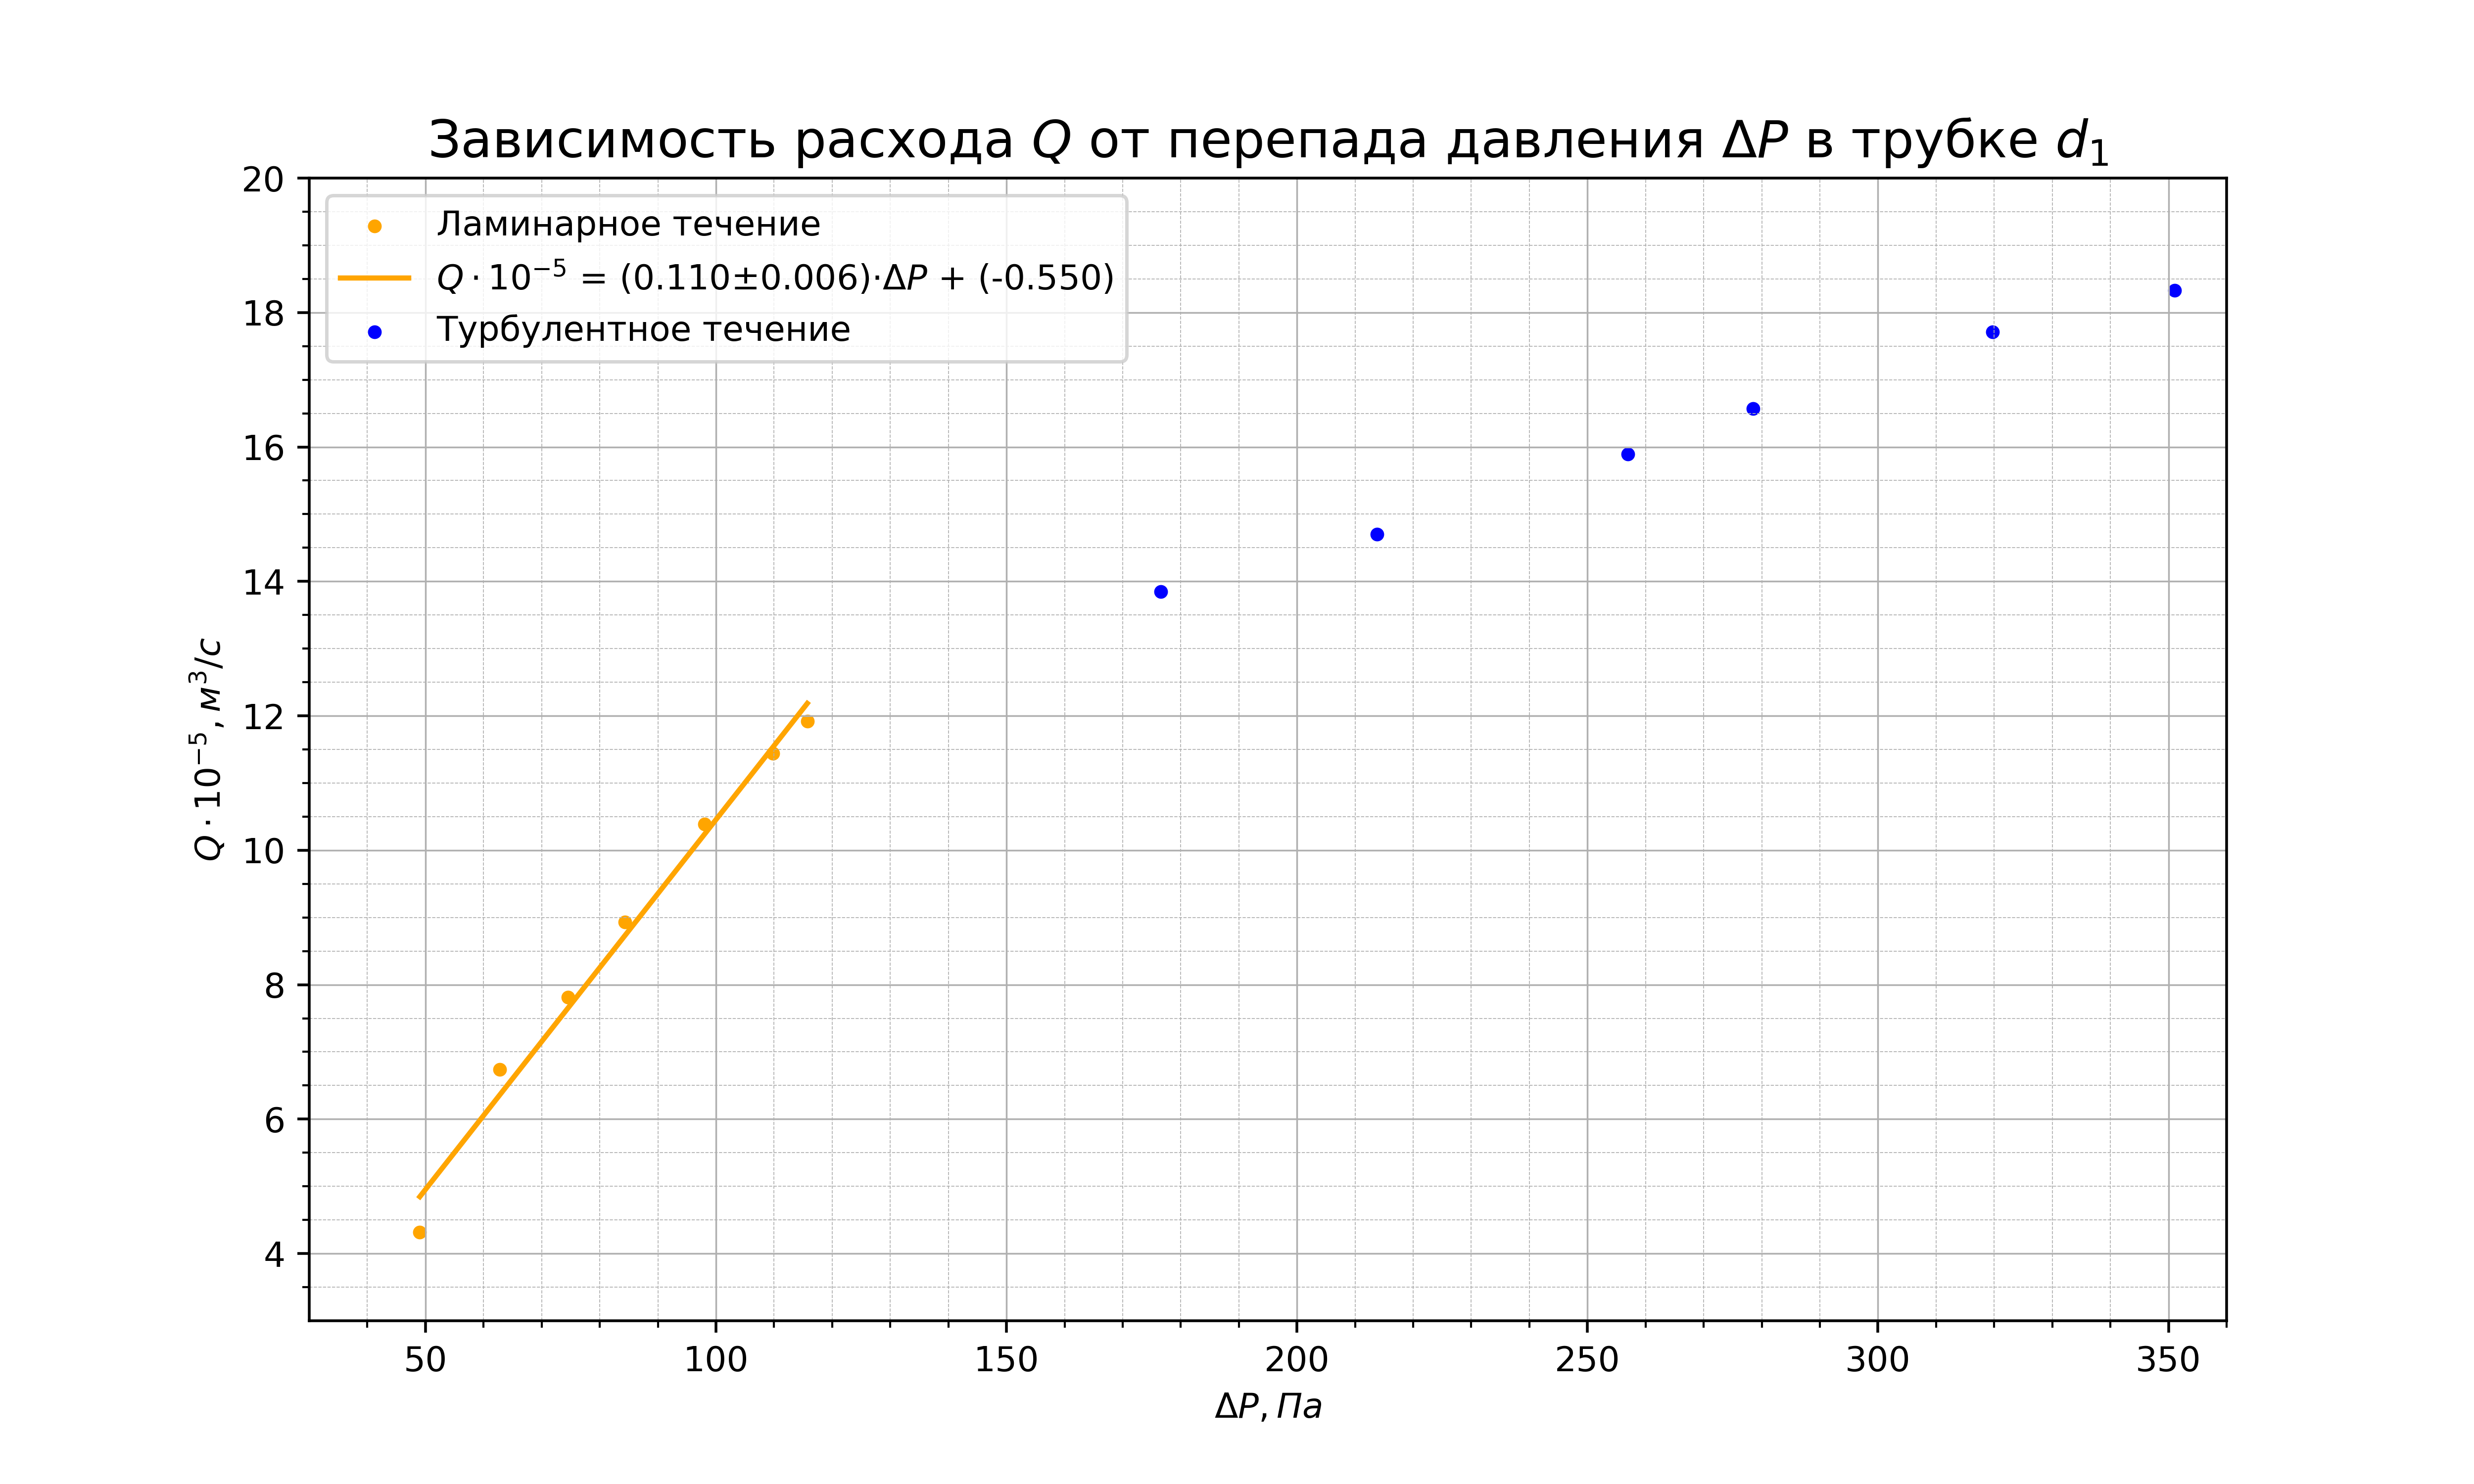
\includegraphics[scale=0.75]{1.3.3_1.png}
\end{flushleft}
\caption{}
\label{ris6}
\end{figure}

\newpage
\par По формуле Пуазейля \eqref{10} определим вязкость воздуха $\eta = \frac{\pi R^4\Delta{P}}{8Ql}$. Погрешность определяется по формуле
\begin{equation}\label{19}
\delta_{\eta} = \sqrt{16\left(\frac{\delta_{R}}{R}\right)^2 + \left(\frac{\delta_{\Delta{P}}}{\Delta{P}}\right)^2 + \left(\frac{\delta_{Q}}{Q}\right)^2} \cdot \eta.
\end{equation}
Полученное значение $\eta = 19,82\pm0,81\cdot10^{-6}$ Па $\cdot$ c.
\par Из формулы \eqref{17} определяем $Re_{\text{кр}}$:
\begin{equation}\label{20}
Re_{\text{кр}} = \frac{Q_{\text{кр}}P_{\text{атм}}\mu}{\eta\pi rRT}.
\end{equation}
Погрешность определяется по формуле:
\begin{equation}\label{21}
\delta_{Re_{\text{кр}}} = \sqrt{\left(\frac{\delta_{Q_{\text{кр}}}}{Q_{\text{кр}}}\right)^2 + \left(\frac{\delta_{P_{\text{атм}}}}{P_{\text{атм}}}\right)^2 + \left(\frac{\delta_{\eta}}{\eta}\right)^2 + \left(\frac{\delta_{T}}{T}\right)^2 + \left(\frac{\delta_{r}}{r}\right)^2} \cdot Re_{\text{кр}}.
\end{equation}
Полученное значение $Re_{\text{кр}} = 919\pm39$.
\par Результаты измерения зависимости $P(x)$ представленны в таблице \ref{tab3}.
\begin{table}[h!]
\begin{center}
\begin{tabular}{|c|c|c|}
\hline
$x$, см & $P(x)$, дел & $P(x)$, Па \\ \hline
40    & 28        & 54,91724 \\ \hline
50    & 32        & 62,76256 \\ \hline
90    & 60        & 117,6798 \\ \hline
120   & 81        & 158,8677 \\ \hline
\end{tabular}
\caption{}
\label{tab3}
\end{center}
\end{table}
Полученный график зависимости представлен на Рис. \ref{ris7}.
\begin{figure}[h!]
\begin{flushleft}
    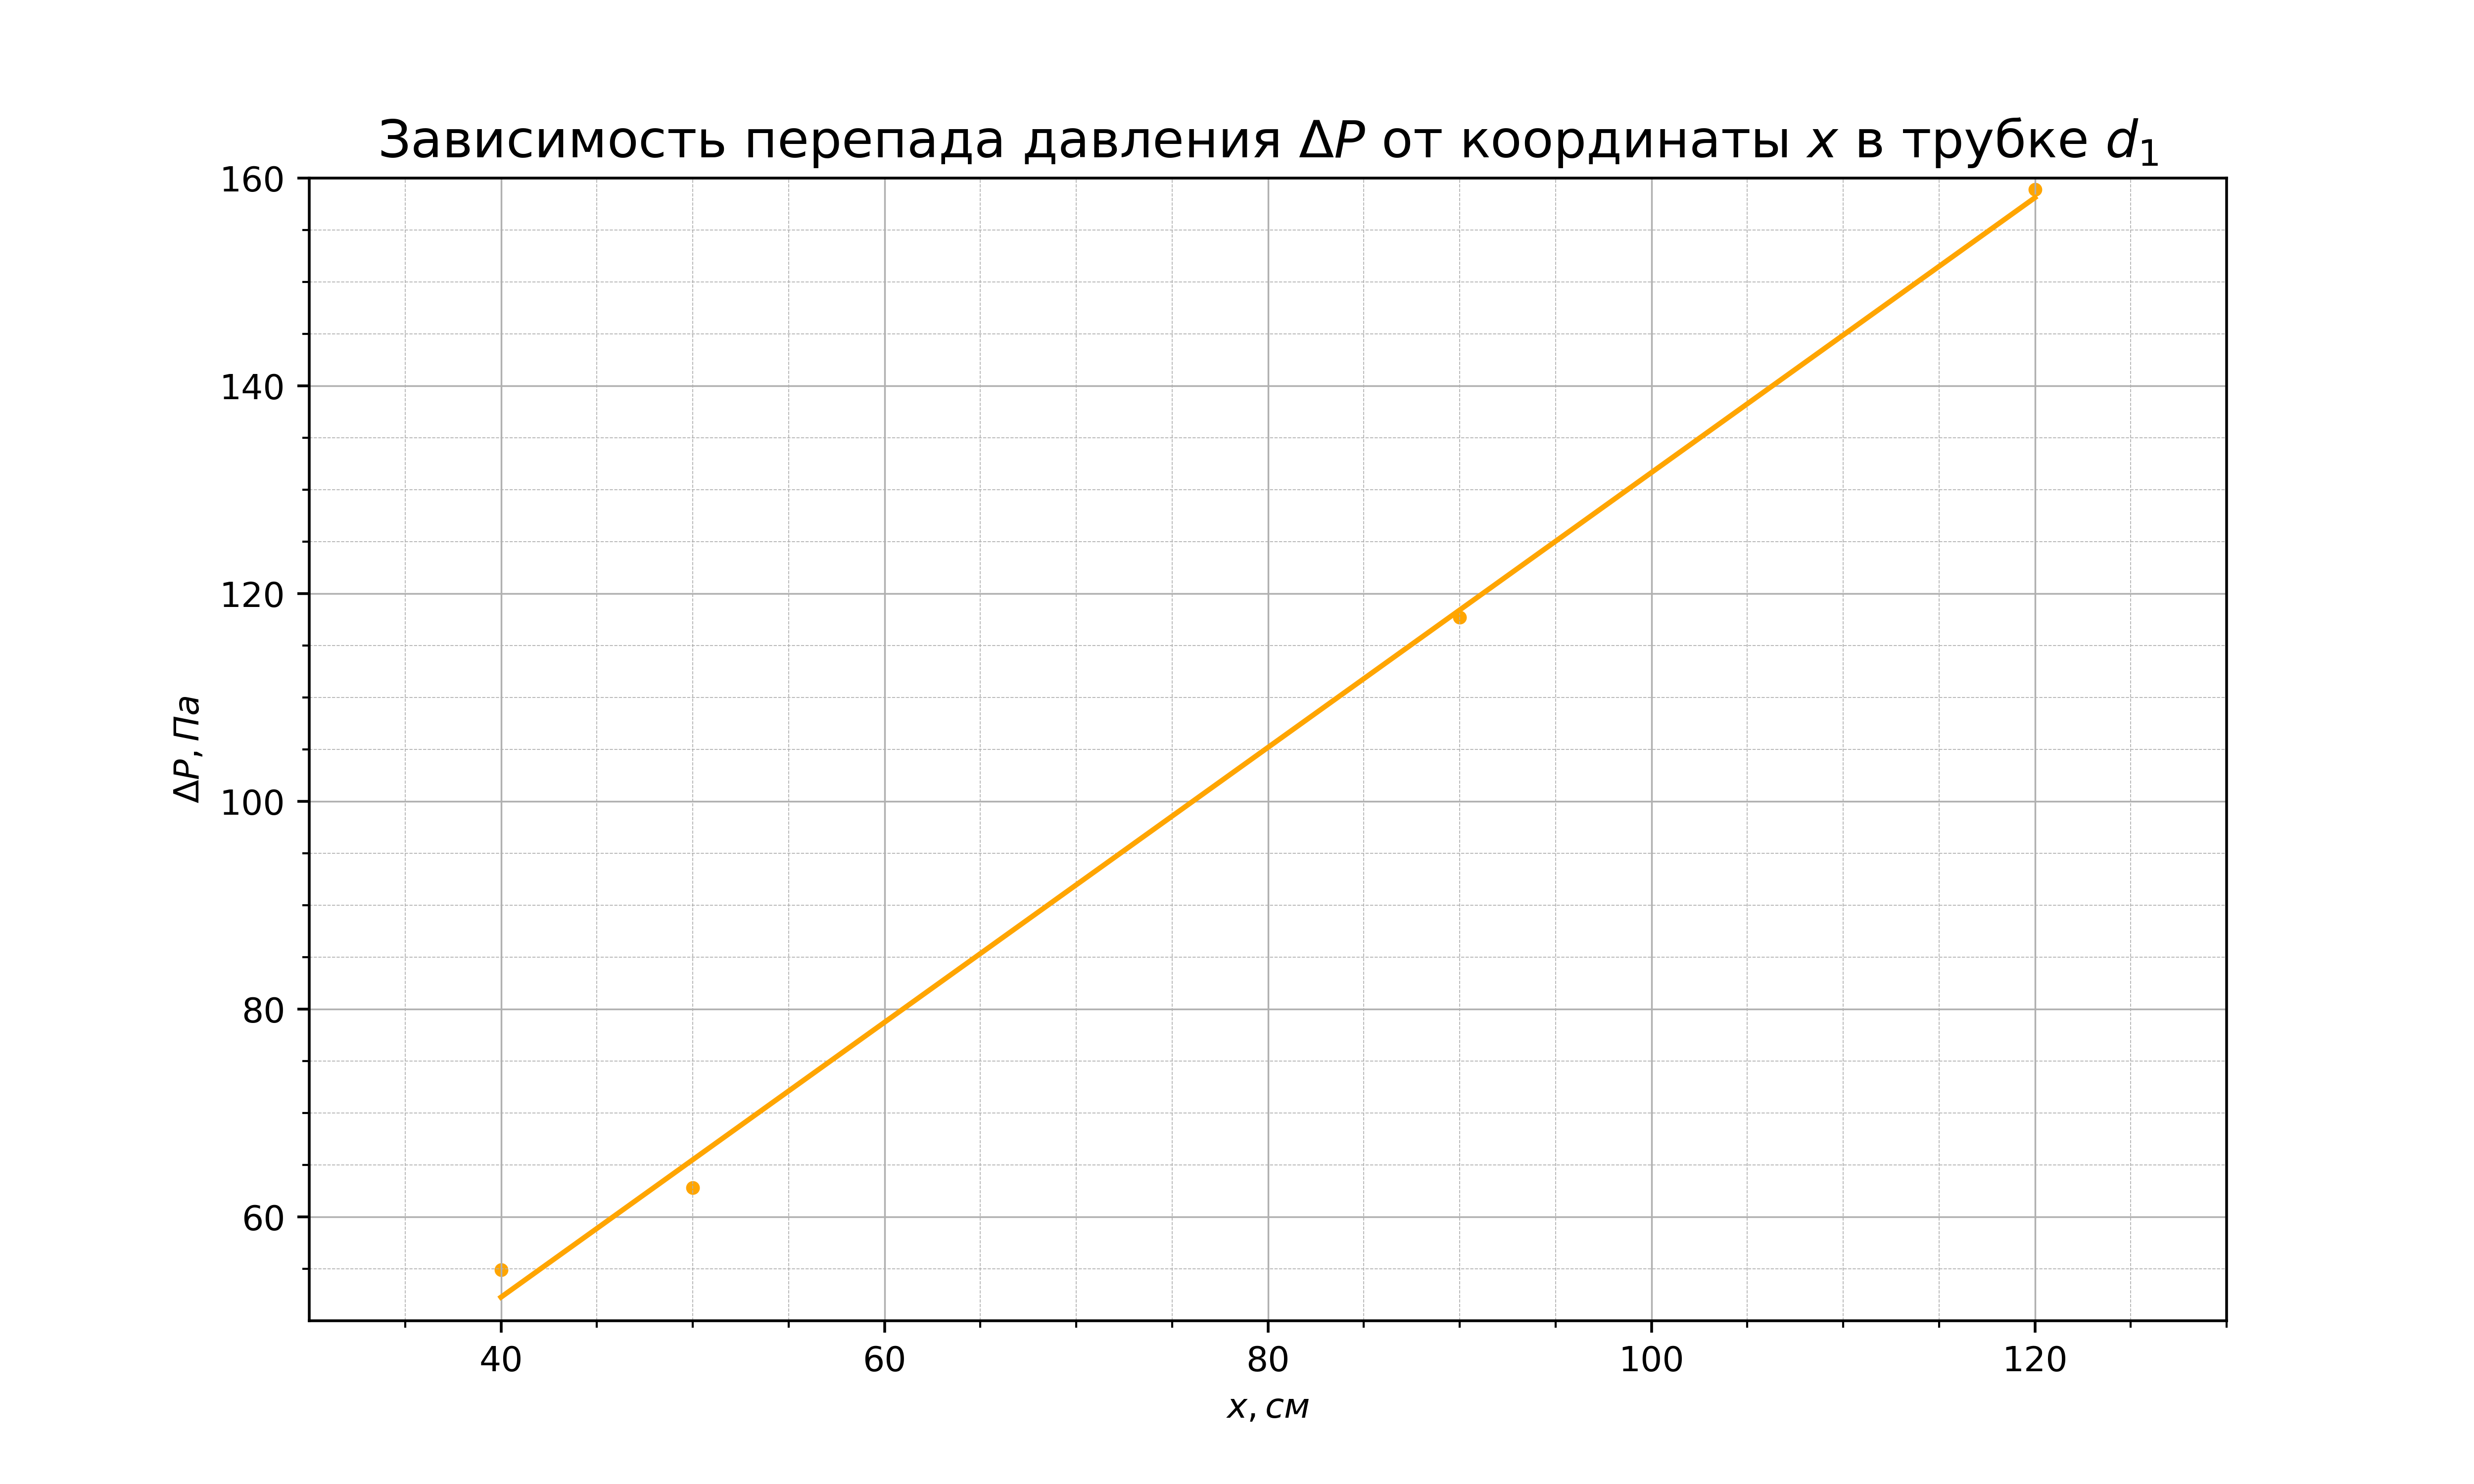
\includegraphics[scale=0.75]{1.3.3_3.png}
\end{flushleft}
\caption{}
\label{ris7}
\end{figure}
Получаем $l_{\text{уст}} \approx 50~\text{см}$, что соотвествует результату, рассчитанному по формуле \eqref{15}.\\[3cm]
\subsection{2 трубка}
\par Проведём предварительные расчёты для второй трубки ($l = 0,5~\text{м}, d_2 = 3,90\pm0,05~\text{мм}$). По формуле \eqref{17} получаем $Q_{\text{кр}} \approx 10,6 \cdot 10^{-5}$ м$^3$/с.
\par По формуле \eqref{18} находим $\Delta{P} \approx 257~\text{Па}$, т. е. 131 деление микроманометра.
\par По формуле \eqref{15} оценим длину $l_{\text{уст}} \approx 0,39~\text{м}$, что меньше длины выбранного участка. Значит, течение можно считать установившимся.

\par Полученные результаты измерения $\Delta{P}(Q)$ при ламинарном течении представленны в таблице \ref{tab4}.
\begin{table}[h!]
\begin{tabular}{|c|c|c|c|c|c|c|c|c|c|}
\hline
$\Delta{P}$, дел    & $\Delta{P}$, Па           & $\delta_{\Delta{P}}$, Па  & $\Delta{t}$, с & $\overline{\Delta{t}}$, c & $\delta_{\overline{\Delta{t}}}$, с & $\Delta{V}$, л     & $\delta_{\Delta{V}}$, л & $Q$, м$^3$/c      & $\delta_{Q}$, м$^3$/с \\ \hline
\multirow{5}{*}{42} & \multirow{5}{*}{82,37586} & \multirow{5}{*}{0,980665} & 17,46 & \multirow{5}{*}{18,67}         & \multirow{5}{*}{0,333581}         & \multirow{5}{*}{1} & \multirow{5}{*}{0,01} & \multirow{5}{*}{0,0000536} & \multirow{5}{*}{0,0000011}   \\ \cline{4-4}
                    &                           &                           & 18,85 &                                &                                   &                    &                       &                            &                              \\ \cline{4-4}
                    &                           &                           & 19,26 &                                &                                   &                    &                       &                            &                              \\ \cline{4-4}
                    &                           &                           & 19,14 &                                &                                   &                    &                       &                            &                              \\ \cline{4-4}
                    &                           &                           & 18,66 &                                &                                   &                    &                       &                            &                              \\ \hline
\multirow{5}{*}{30} & \multirow{5}{*}{58,8399}  & \multirow{5}{*}{0,980665} & 28,42 & \multirow{5}{*}{28,11}         & \multirow{5}{*}{0,656277}         & \multirow{5}{*}{1} & \multirow{5}{*}{0,01} & \multirow{5}{*}{0,0000356} & \multirow{5}{*}{0,0000009}   \\ \cline{4-4}
                    &                           &                           & 29,94 &                                &                                   &                    &                       &                            &                              \\ \cline{4-4}
                    &                           &                           & 28,90 &                                &                                   &                    &                       &                            &                              \\ \cline{4-4}
                    &                           &                           & 26,86 &                                &                                   &                    &                       &                            &                              \\ \cline{4-4}
                    &                           &                           & 26,43 &                                &                                   &                    &                       &                            &                              \\ \hline
\multirow{5}{*}{21} & \multirow{5}{*}{41,18793} & \multirow{5}{*}{0,980665} & 41,88 & \multirow{5}{*}{38,80}         & \multirow{5}{*}{0,985132}         & \multirow{5}{*}{1} & \multirow{5}{*}{0,01} & \multirow{5}{*}{0,0000258} & \multirow{5}{*}{0,0000007}   \\ \cline{4-4}
                    &                           &                           & 39,58 &                                &                                   &                    &                       &                            &                              \\ \cline{4-4}
                    &                           &                           & 36,43 &                                &                                   &                    &                       &                            &                              \\ \cline{4-4}
                    &                           &                           & 36,95 &                                &                                   &                    &                       &                            &                              \\ \cline{4-4}
                    &                           &                           & 39,14 &                                &                                   &                    &                       &                            &                              \\ \hline
\multirow{5}{*}{51} & \multirow{5}{*}{100,0278} & \multirow{5}{*}{0,980665} & 16,85 & \multirow{5}{*}{17,08}         & \multirow{5}{*}{0,421172}         & \multirow{5}{*}{1} & \multirow{5}{*}{0,01} & \multirow{5}{*}{0,0000586} & \multirow{5}{*}{0,0000016}   \\ \cline{4-4}
                    &                           &                           & 15,66 &                                &                                   &                    &                       &                            &                              \\ \cline{4-4}
                    &                           &                           & 17,15 &                                &                                   &                    &                       &                            &                              \\ \cline{4-4}
                    &                           &                           & 18,08 &                                &                                   &                    &                       &                            &                              \\ \cline{4-4}
                    &                           &                           & 17,64 &                                &                                   &                    &                       &                            &                              \\ \hline
\multirow{5}{*}{62} & \multirow{5}{*}{121,6025} & \multirow{5}{*}{0,980665} & 14,59 & \multirow{5}{*}{14,20}         & \multirow{5}{*}{0,359166}         & \multirow{5}{*}{1} & \multirow{5}{*}{0,01} & \multirow{5}{*}{0,0000704} & \multirow{5}{*}{0,0000019}   \\ \cline{4-4}
                    &                           &                           & 15,15 &                                &                                   &                    &                       &                            &                              \\ \cline{4-4}
                    &                           &                           & 14,41 &                                &                                   &                    &                       &                            &                              \\ \cline{4-4}
                    &                           &                           & 13,67 &                                &                                   &                    &                       &                            &                              \\ \cline{4-4}
                    &                           &                           & 13,18 &                                &                                   &                    &                       &                            &                              \\ \hline
\multirow{5}{*}{56} & \multirow{5}{*}{109,8345} & \multirow{5}{*}{0,980665} & 14,71 & \multirow{5}{*}{15,41}         & \multirow{5}{*}{0,285594}         & \multirow{5}{*}{1} & \multirow{5}{*}{0,01} & \multirow{5}{*}{0,0000649} & \multirow{5}{*}{0,0000014}   \\ \cline{4-4}
                    &                           &                           & 15,23 &                                &                                   &                    &                       &                            &                              \\ \cline{4-4}
                    &                           &                           & 16,24 &                                &                                   &                    &                       &                            &                              \\ \cline{4-4}
                    &                           &                           & 15,79 &                                &                                   &                    &                       &                            &                              \\ \cline{4-4}
                    &                           &                           & 15,07 &                                &                                   &                    &                       &                            &                              \\ \hline
\multirow{5}{*}{66} & \multirow{5}{*}{129,4478} & \multirow{5}{*}{0,980665} & 13,75 & \multirow{5}{*}{13,16}         & \multirow{5}{*}{0,238273}         & \multirow{5}{*}{1} & \multirow{5}{*}{0,01} & \multirow{5}{*}{0,0000760} & \multirow{5}{*}{0,0000016}   \\ \cline{4-4}
                    &                           &                           & 13,08 &                                &                                   &                    &                       &                            &                              \\ \cline{4-4}
                    &                           &                           & 12,48 &                                &                                   &                    &                       &                            &                              \\ \cline{4-4}
                    &                           &                           & 12,97 &                                &                                   &                    &                       &                            &                              \\ \cline{4-4}
                    &                           &                           & 13,51 &                                &                                   &                    &                       &                            &                              \\ \hline
\end{tabular}
\caption{Ламинарное течение}
\label{tab4}
\end{table}

\newpage
\par Полученные результаты измерения $\Delta{P}(Q)$ при турбулентном течении представленны в таблице \ref{tab5}.
\begin{table}[h!]
\begin{tabular}{|c|c|c|c|c|c|c|c|c|c|}
\hline
$\Delta{P}$, дел    & $\Delta{P}$, Па           & $\delta_{\Delta{P}}$, Па  & $\Delta{t}$, с & $\overline{\Delta{t}}$, c & $\delta_{\overline{\Delta{t}}}$, с & $\Delta{V}$, л     & $\delta_{\Delta{V}}$, л & $Q$, м$^3$/c      & $\delta_{Q}$, м$^3$/с \\ \hline
\multirow{5}{*}{80}  & \multirow{5}{*}{156,9064} & \multirow{5}{*}{0,980665} & 11,88 & \multirow{5}{*}{11,37}         & \multirow{5}{*}{0,230078}         & \multirow{5}{*}{1} & \multirow{5}{*}{0,01} & \multirow{5}{*}{0,0000880} & \multirow{5}{*}{0,0000020}   \\ \cline{4-4}
                     &                           &                           & 10,93 &                                &                                   &                    &                       &                            &                              \\ \cline{4-4}
                     &                           &                           & 10,86 &                                &                                   &                    &                       &                            &                              \\ \cline{4-4}
                     &                           &                           & 11,36 &                                &                                   &                    &                       &                            &                              \\ \cline{4-4}
                     &                           &                           & 11,80 &                                &                                   &                    &                       &                            &                              \\ \hline
\multirow{5}{*}{121} & \multirow{5}{*}{237,3209} & \multirow{5}{*}{0,980665} & 9,66  & \multirow{5}{*}{9,72}          & \multirow{5}{*}{0,265714}         & \multirow{5}{*}{1} & \multirow{5}{*}{0,01} & \multirow{5}{*}{0,0001029} & \multirow{5}{*}{0,0000030}   \\ \cline{4-4}
                     &                           &                           & 8,78  &                                &                                   &                    &                       &                            &                              \\ \cline{4-4}
                     &                           &                           & 9,93  &                                &                                   &                    &                       &                            &                              \\ \cline{4-4}
                     &                           &                           & 10,10 &                                &                                   &                    &                       &                            &                              \\ \cline{4-4}
                     &                           &                           & 10,14 &                                &                                   &                    &                       &                            &                              \\ \hline
\multirow{5}{*}{144} & \multirow{5}{*}{282,4315} & \multirow{5}{*}{0,980665} & 9,06  & \multirow{5}{*}{8,99}          & \multirow{5}{*}{0,177104}         & \multirow{5}{*}{1} & \multirow{5}{*}{0,01} & \multirow{5}{*}{0,0001113} & \multirow{5}{*}{0,0000025}   \\ \cline{4-4}
                     &                           &                           & 9,26  &                                &                                   &                    &                       &                            &                              \\ \cline{4-4}
                     &                           &                           & 9,35  &                                &                                   &                    &                       &                            &                              \\ \cline{4-4}
                     &                           &                           & 8,61  &                                &                                   &                    &                       &                            &                              \\ \cline{4-4}
                     &                           &                           & 8,65  &                                &                                   &                    &                       &                            &                              \\ \hline
\multirow{5}{*}{178} & \multirow{5}{*}{349,1167} & \multirow{5}{*}{0,980665} & 7,63  & \multirow{5}{*}{8,20}          & \multirow{5}{*}{0,187286}         & \multirow{5}{*}{1} & \multirow{5}{*}{0,01} & \multirow{5}{*}{0,0001219} & \multirow{5}{*}{0,0000030}   \\ \cline{4-4}
                     &                           &                           & 8,21  &                                &                                   &                    &                       &                            &                              \\ \cline{4-4}
                     &                           &                           & 8,54  &                                &                                   &                    &                       &                            &                              \\ \cline{4-4}
                     &                           &                           & 8,51  &                                &                                   &                    &                       &                            &                              \\ \cline{4-4}
                     &                           &                           & 8,13  &                                &                                   &                    &                       &                            &                              \\ \hline
\multirow{5}{*}{206} & \multirow{5}{*}{404,034}  & \multirow{5}{*}{0,980665} & 7,35  & \multirow{5}{*}{7,67}          & \multirow{5}{*}{0,157067}         & \multirow{5}{*}{1} & \multirow{5}{*}{0,01} & \multirow{5}{*}{0,0001304} & \multirow{5}{*}{0,0000030}   \\ \cline{4-4}
                     &                           &                           & 7,63  &                                &                                   &                    &                       &                            &                              \\ \cline{4-4}
                     &                           &                           & 8,00  &                                &                                   &                    &                       &                            &                              \\ \cline{4-4}
                     &                           &                           & 7,93  &                                &                                   &                    &                       &                            &                              \\ \cline{4-4}
                     &                           &                           & 7,44  &                                &                                   &                    &                       &                            &                              \\ \hline
\multirow{5}{*}{83}  & \multirow{5}{*}{162,7904} & \multirow{5}{*}{0,980665} & 10,95 & \multirow{5}{*}{11,27}         & \multirow{5}{*}{0,29416}          & \multirow{5}{*}{1} & \multirow{5}{*}{0,01} & \multirow{5}{*}{0,0000887} & \multirow{5}{*}{0,0000025}   \\ \cline{4-4}
                     &                           &                           & 10,51 &                                &                                   &                    &                       &                            &                              \\ \cline{4-4}
                     &                           &                           & 11,06 &                                &                                   &                    &                       &                            &                              \\ \cline{4-4}
                     &                           &                           & 12,00 &                                &                                   &                    &                       &                            &                              \\ \cline{4-4}
                     &                           &                           & 11,83 &                                &                                   &                    &                       &                            &                              \\ \hline
\multirow{5}{*}{101} & \multirow{5}{*}{198,0943} & \multirow{5}{*}{0,980665} & 10,79 & \multirow{5}{*}{10,47}         & \multirow{5}{*}{0,21421}          & \multirow{5}{*}{1} & \multirow{5}{*}{0,01} & \multirow{5}{*}{0,0000955} & \multirow{5}{*}{0,0000022}   \\ \cline{4-4}
                     &                           &                           & 10,38 &                                &                                   &                    &                       &                            &                              \\ \cline{4-4}
                     &                           &                           & 9,81  &                                &                                   &                    &                       &                            &                              \\ \cline{4-4}
                     &                           &                           & 10,46 &                                &                                   &                    &                       &                            &                              \\ \cline{4-4}
                     &                           &                           & 10,93 &                                &                                   &                    &                       &                            &                              \\ \hline
\end{tabular}
\caption{Турбулентное течение}
\label{tab5}
\end{table}

\newpage
\par Полученный график зависимости $Q(\Delta{P})$ представлен на Рис. \ref{ris8}.
\begin{figure}[h!]
\begin{flushleft}
    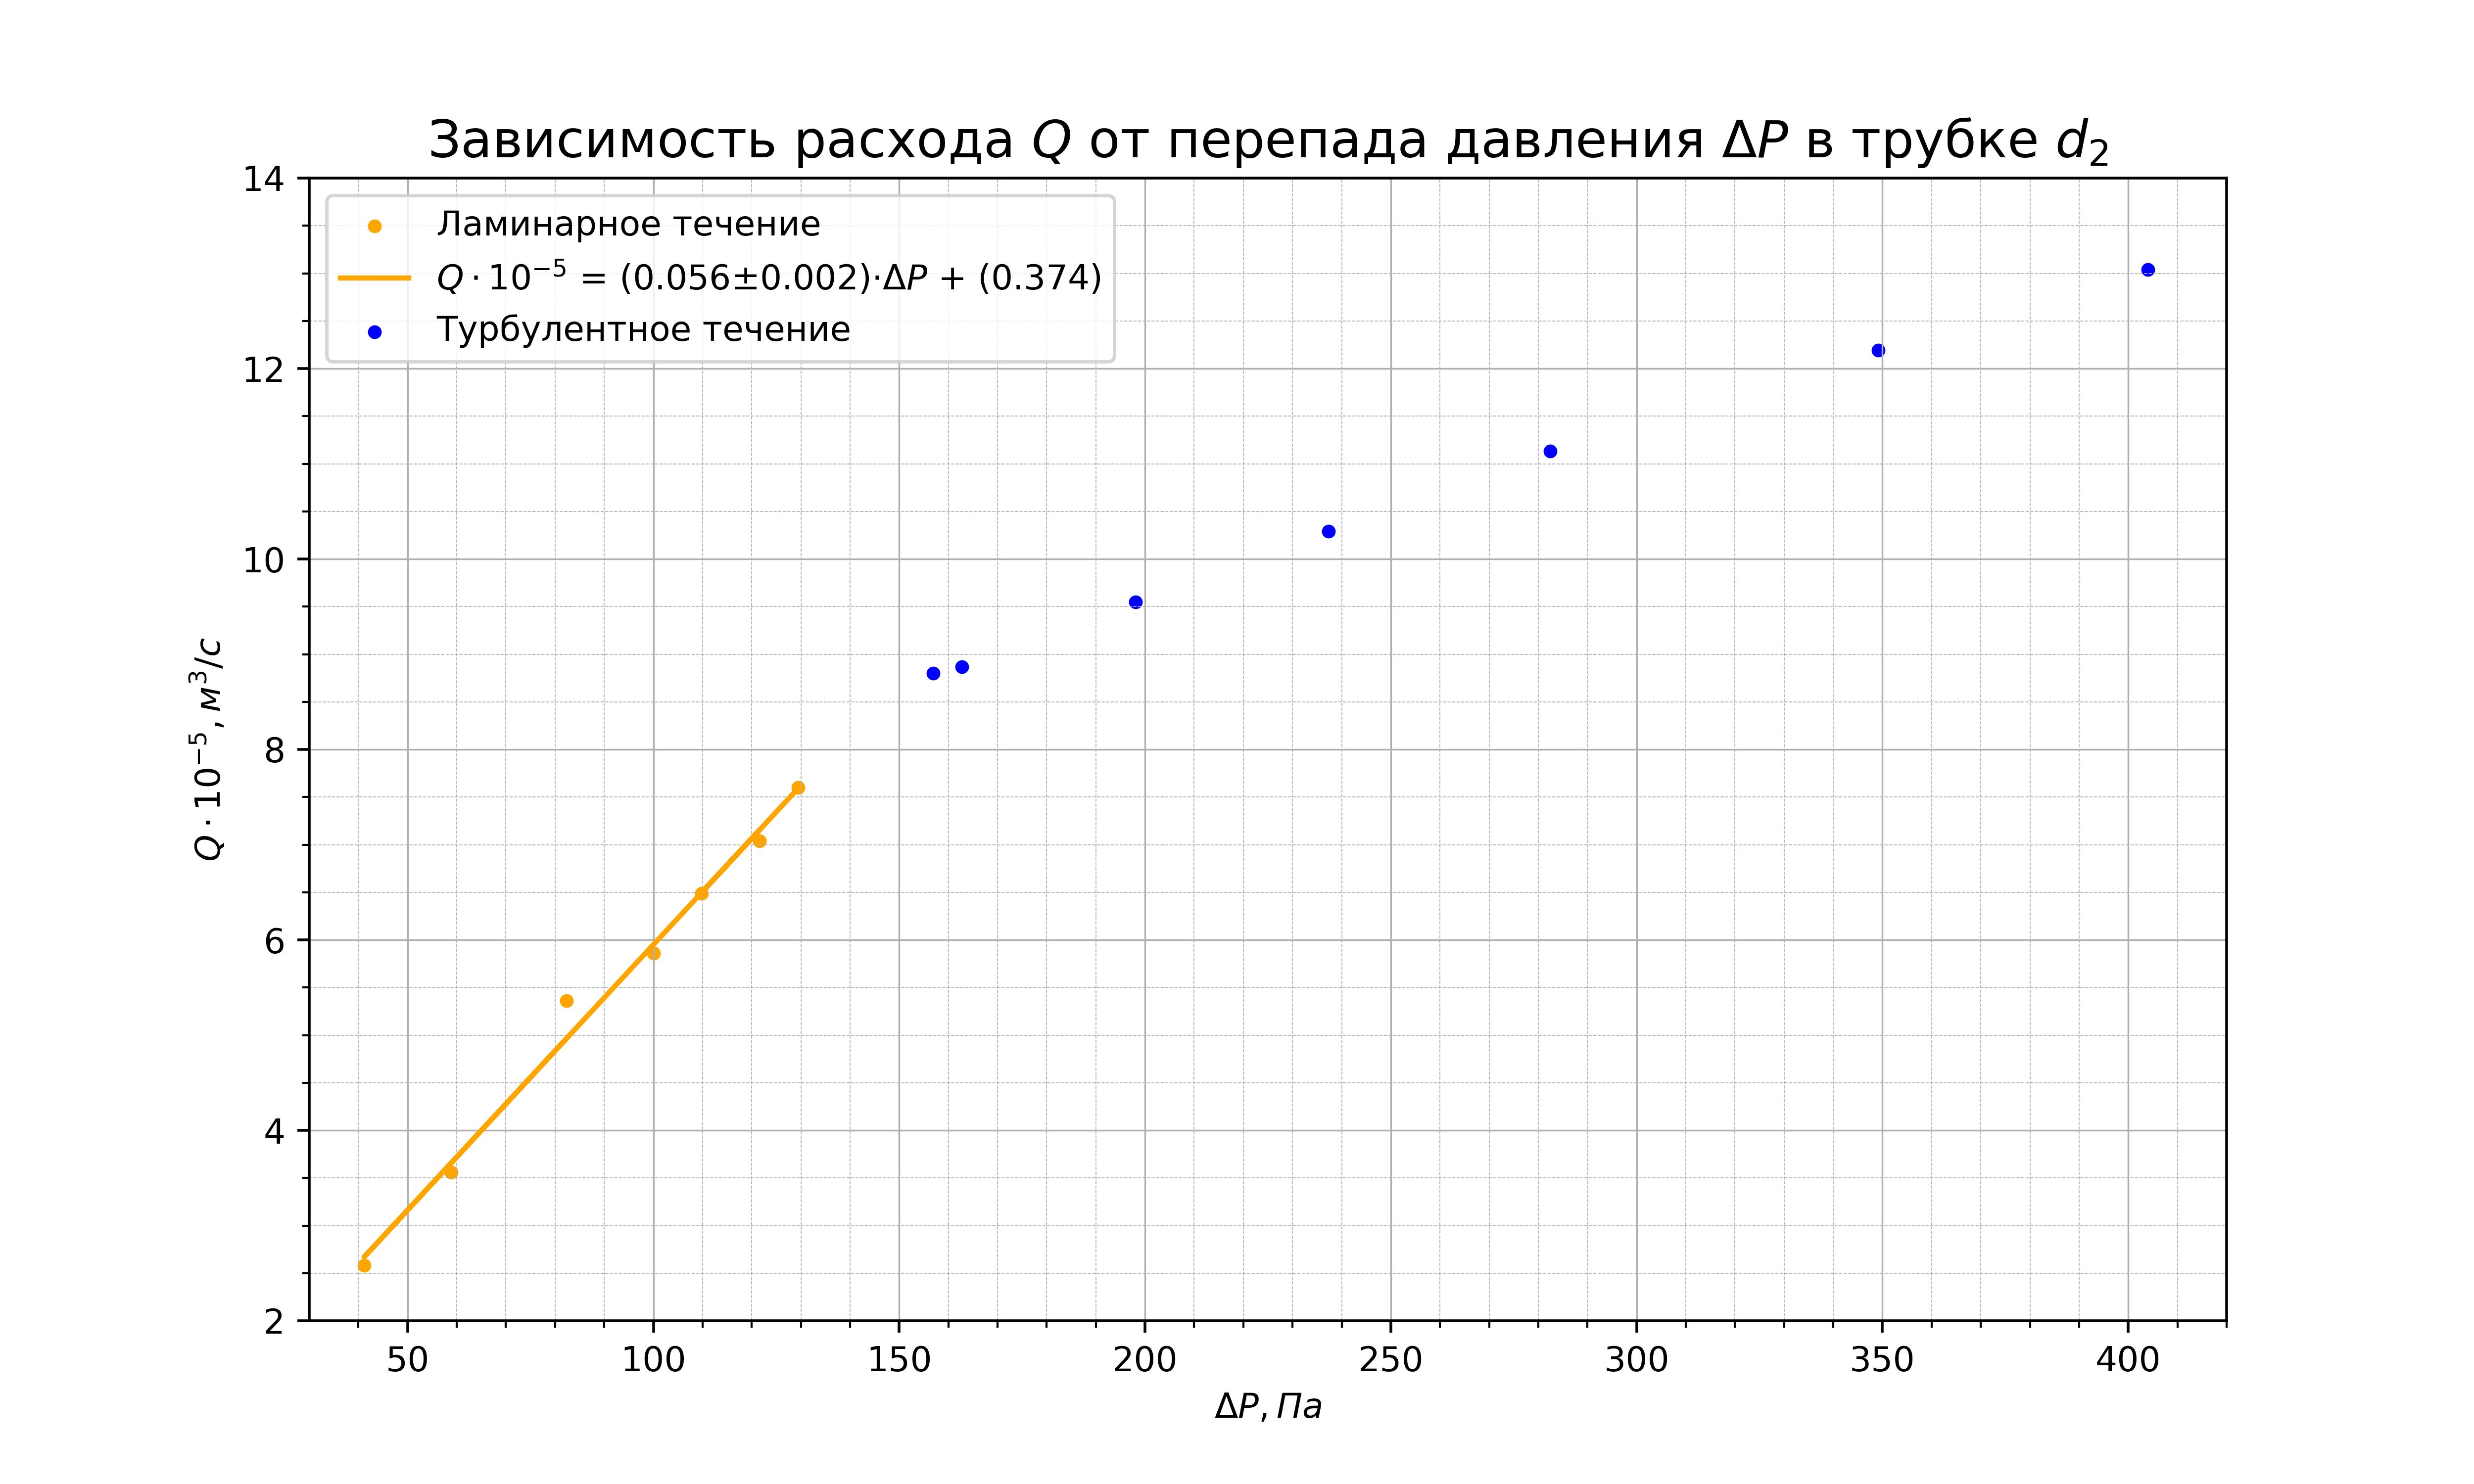
\includegraphics[scale=0.75]{1.3.3_2.png}
\end{flushleft}
\caption{}
\label{ris8}
\end{figure}

\newpage
\par По формуле Пуазейля \eqref{10} определим вязкость воздуха $\eta = \frac{\pi R^4\Delta{P}}{8Ql}$. Погрешность определяется по формуле \eqref{19}.
Полученное значение $\eta = 19,01\pm1,01\cdot10^{-6}$ Па $\cdot$ c.
\par По формулам \eqref{20} и \eqref{21} получаем $Re_{\text{кр}} = 844\pm47$:
\par Результаты измерения зависимости $P(x)$ представленны в таблице \ref{tab6}.
\begin{table}[h!]
\begin{center}
\begin{tabular}{|c|c|c|}
\hline
$x$, см & $P(x)$, дел & $P(x)$, Па \\ \hline
50    & 75        & 147,0998 \\ \hline
90    & 135       & 264,7796 \\ \hline
120   & 184       & 360,8847 \\ \hline
\end{tabular}
\caption{}
\label{tab6}
\end{center}
\end{table}
Полученный график зависимости представлен на Рис. \ref{ris9}.
\begin{figure}[h!]
\begin{flushleft}
    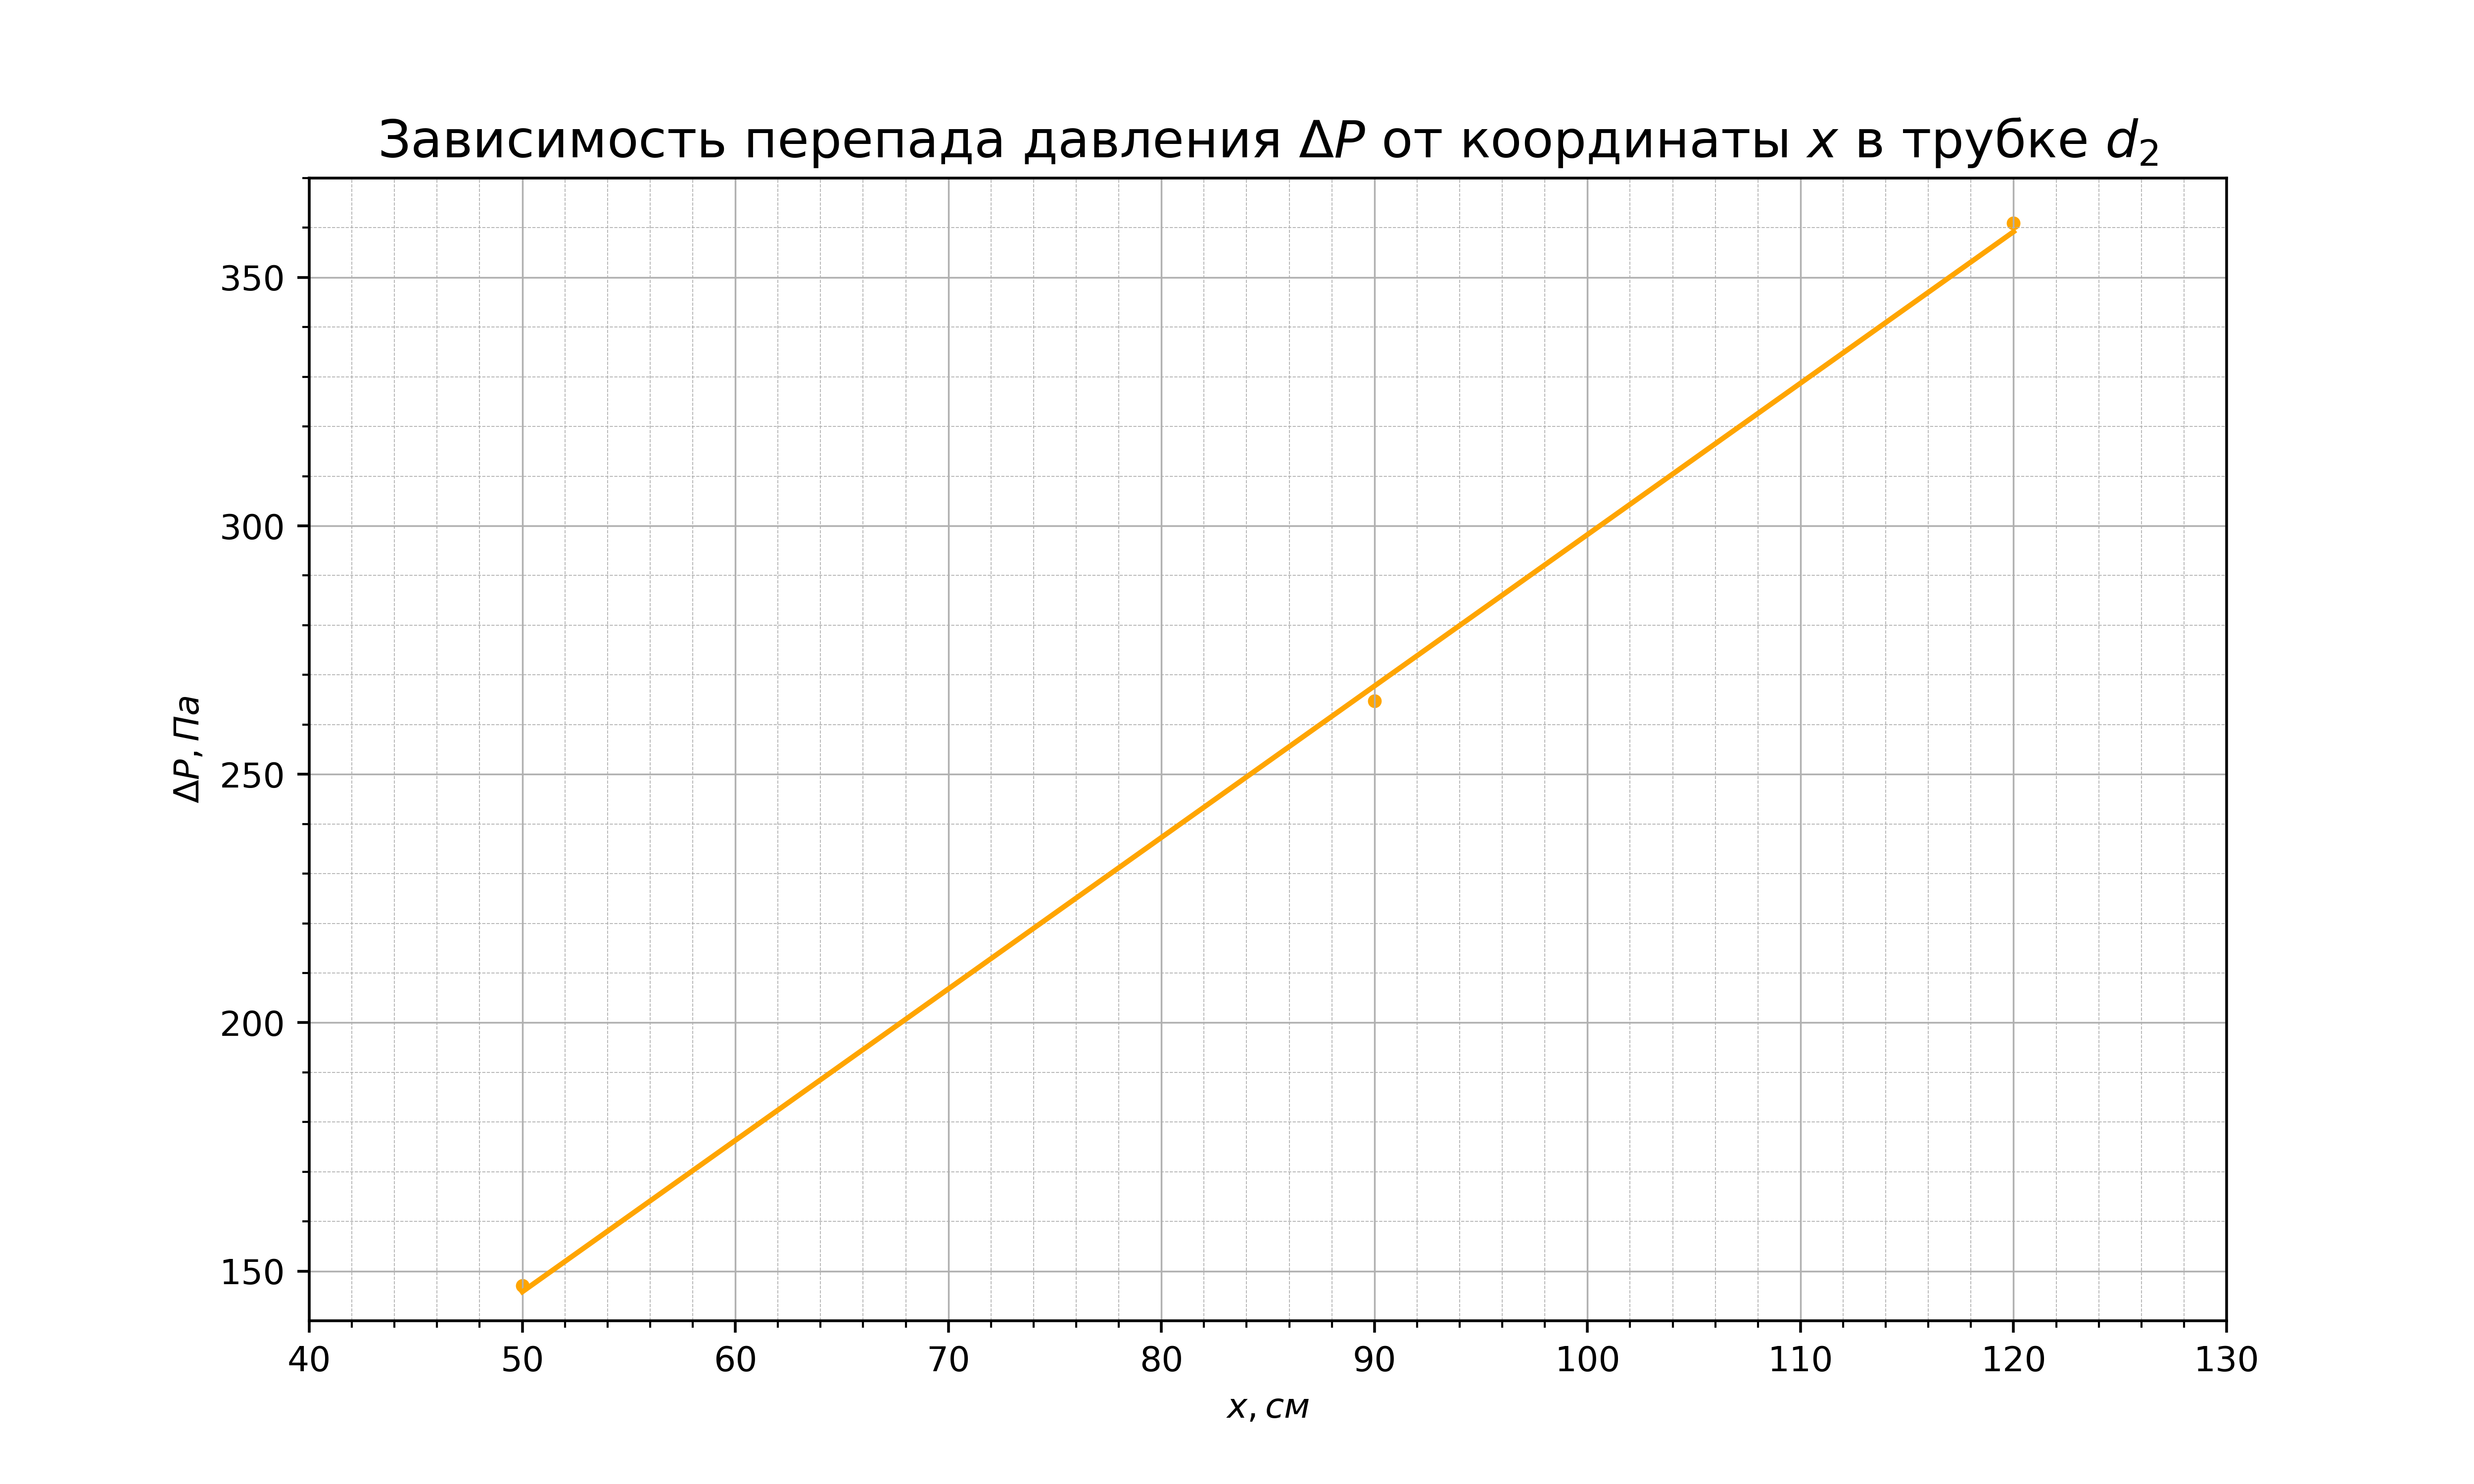
\includegraphics[scale=0.75]{1.3.3_4.png}
\end{flushleft}
\caption{}
\label{ris9}
\end{figure}
Получаем $l_{\text{уст}} \approx 40~\text{см}$, что соотвествует результату, рассчитанному по формуле \eqref{15}.\\[6cm]

\par Измерения зависимости расхода от радиуса трубы при заданном градиенте $\frac{\Delta{P}}{l} = \frac{2}{3}\frac{дел}{см}$ (ламинарное течение) представленны в таблице \ref{tab7}.
\begin{table}[h!]
\begin{center}
\begin{tabular}{|c|c|c|c|c|}
\hline
 & $\Delta{t}, c$ & $\overline{\Delta{t}}, c$ & $\Delta{V}, л$  & $Q, м^3/c$   \\ \hline
\multirow{5}{*}{$d_1$} & 8,77  & \multirow{5}{*}{8,37}          & \multirow{5}{*}{1} & \multirow{5}{*}{0,0001195} \\ \cline{2-2}
                    & 8,23  &                                &                    &                            \\ \cline{2-2}
                    & 8,11  &                                &                    &                            \\ \cline{2-2}
                    & 8,08  &                                &                    &                            \\ \cline{2-2}
                    & 8,66  &                                &                    &                            \\ \hline
\multirow{5}{*}{$d_2$} & 23,9  & \multirow{5}{*}{24,592}        & \multirow{5}{*}{1} & \multirow{5}{*}{0,0000407} \\ \cline{2-2}
                    & 24,43 &                                &                    &                            \\ \cline{2-2}
                    & 24,33 &                                &                    &                            \\ \cline{2-2}
                    & 24,2  &                                &                    &                            \\ \cline{2-2}
                    & 26,1  &                                &                    &                            \\ \hline
\end{tabular}
\caption{Ламинарное течение}
\label{tab7}
\end{center}
\end{table}
\par Измерения зависимости расхода от радиуса трубы при заданном градиенте $\frac{\Delta{P}}{l} = 3\frac{дел}{см}$ (турбулентное течение) представленны в таблице \ref{tab8}.
\begin{table}[h!]
\begin{center}
\begin{tabular}{|c|c|c|c|c|}
\hline
 & $\Delta{t}, c$ & $\overline{\Delta{t}}, c$ & $\Delta{V}, л$  & $Q, м^3/c$ \\ \hline
\multirow{5}{*}{$d_1$} & 4,06  & \multirow{5}{*}{4,306}         & \multirow{5}{*}{1} & \multirow{5}{*}{0,0002322} \\ \cline{2-2}
                    & 4,42  &                                &                    &                            \\ \cline{2-2}
                    & 4,36  &                                &                    &                            \\ \cline{2-2}
                    & 4,63  &                                &                    &                            \\ \cline{2-2}
                    & 4,06  &                                &                    &                            \\ \hline
\multirow{5}{*}{$d_2$} & 9,43  & \multirow{5}{*}{9,028}         & \multirow{5}{*}{1} & \multirow{5}{*}{0,0001108} \\ \cline{2-2}
                    & 9,03  &                                &                    &                            \\ \cline{2-2}
                    & 8,5   &                                &                    &                            \\ \cline{2-2}
                    & 8,9   &                                &                    &                            \\ \cline{2-2}
                    & 9,28  &                                &                    &                            \\ \hline
\end{tabular}
\caption{Турбулентное течение}
\label{tab8}
\end{center}
\end{table}
\par Графики зависимостей $\ln{Q}(\ln{R})$ представленны на Рис. \ref{ris10}. Коэффициент при $x$ прямой будет являться искомым показателем степени.
\begin{figure}[h!]
\begin{flushleft}
    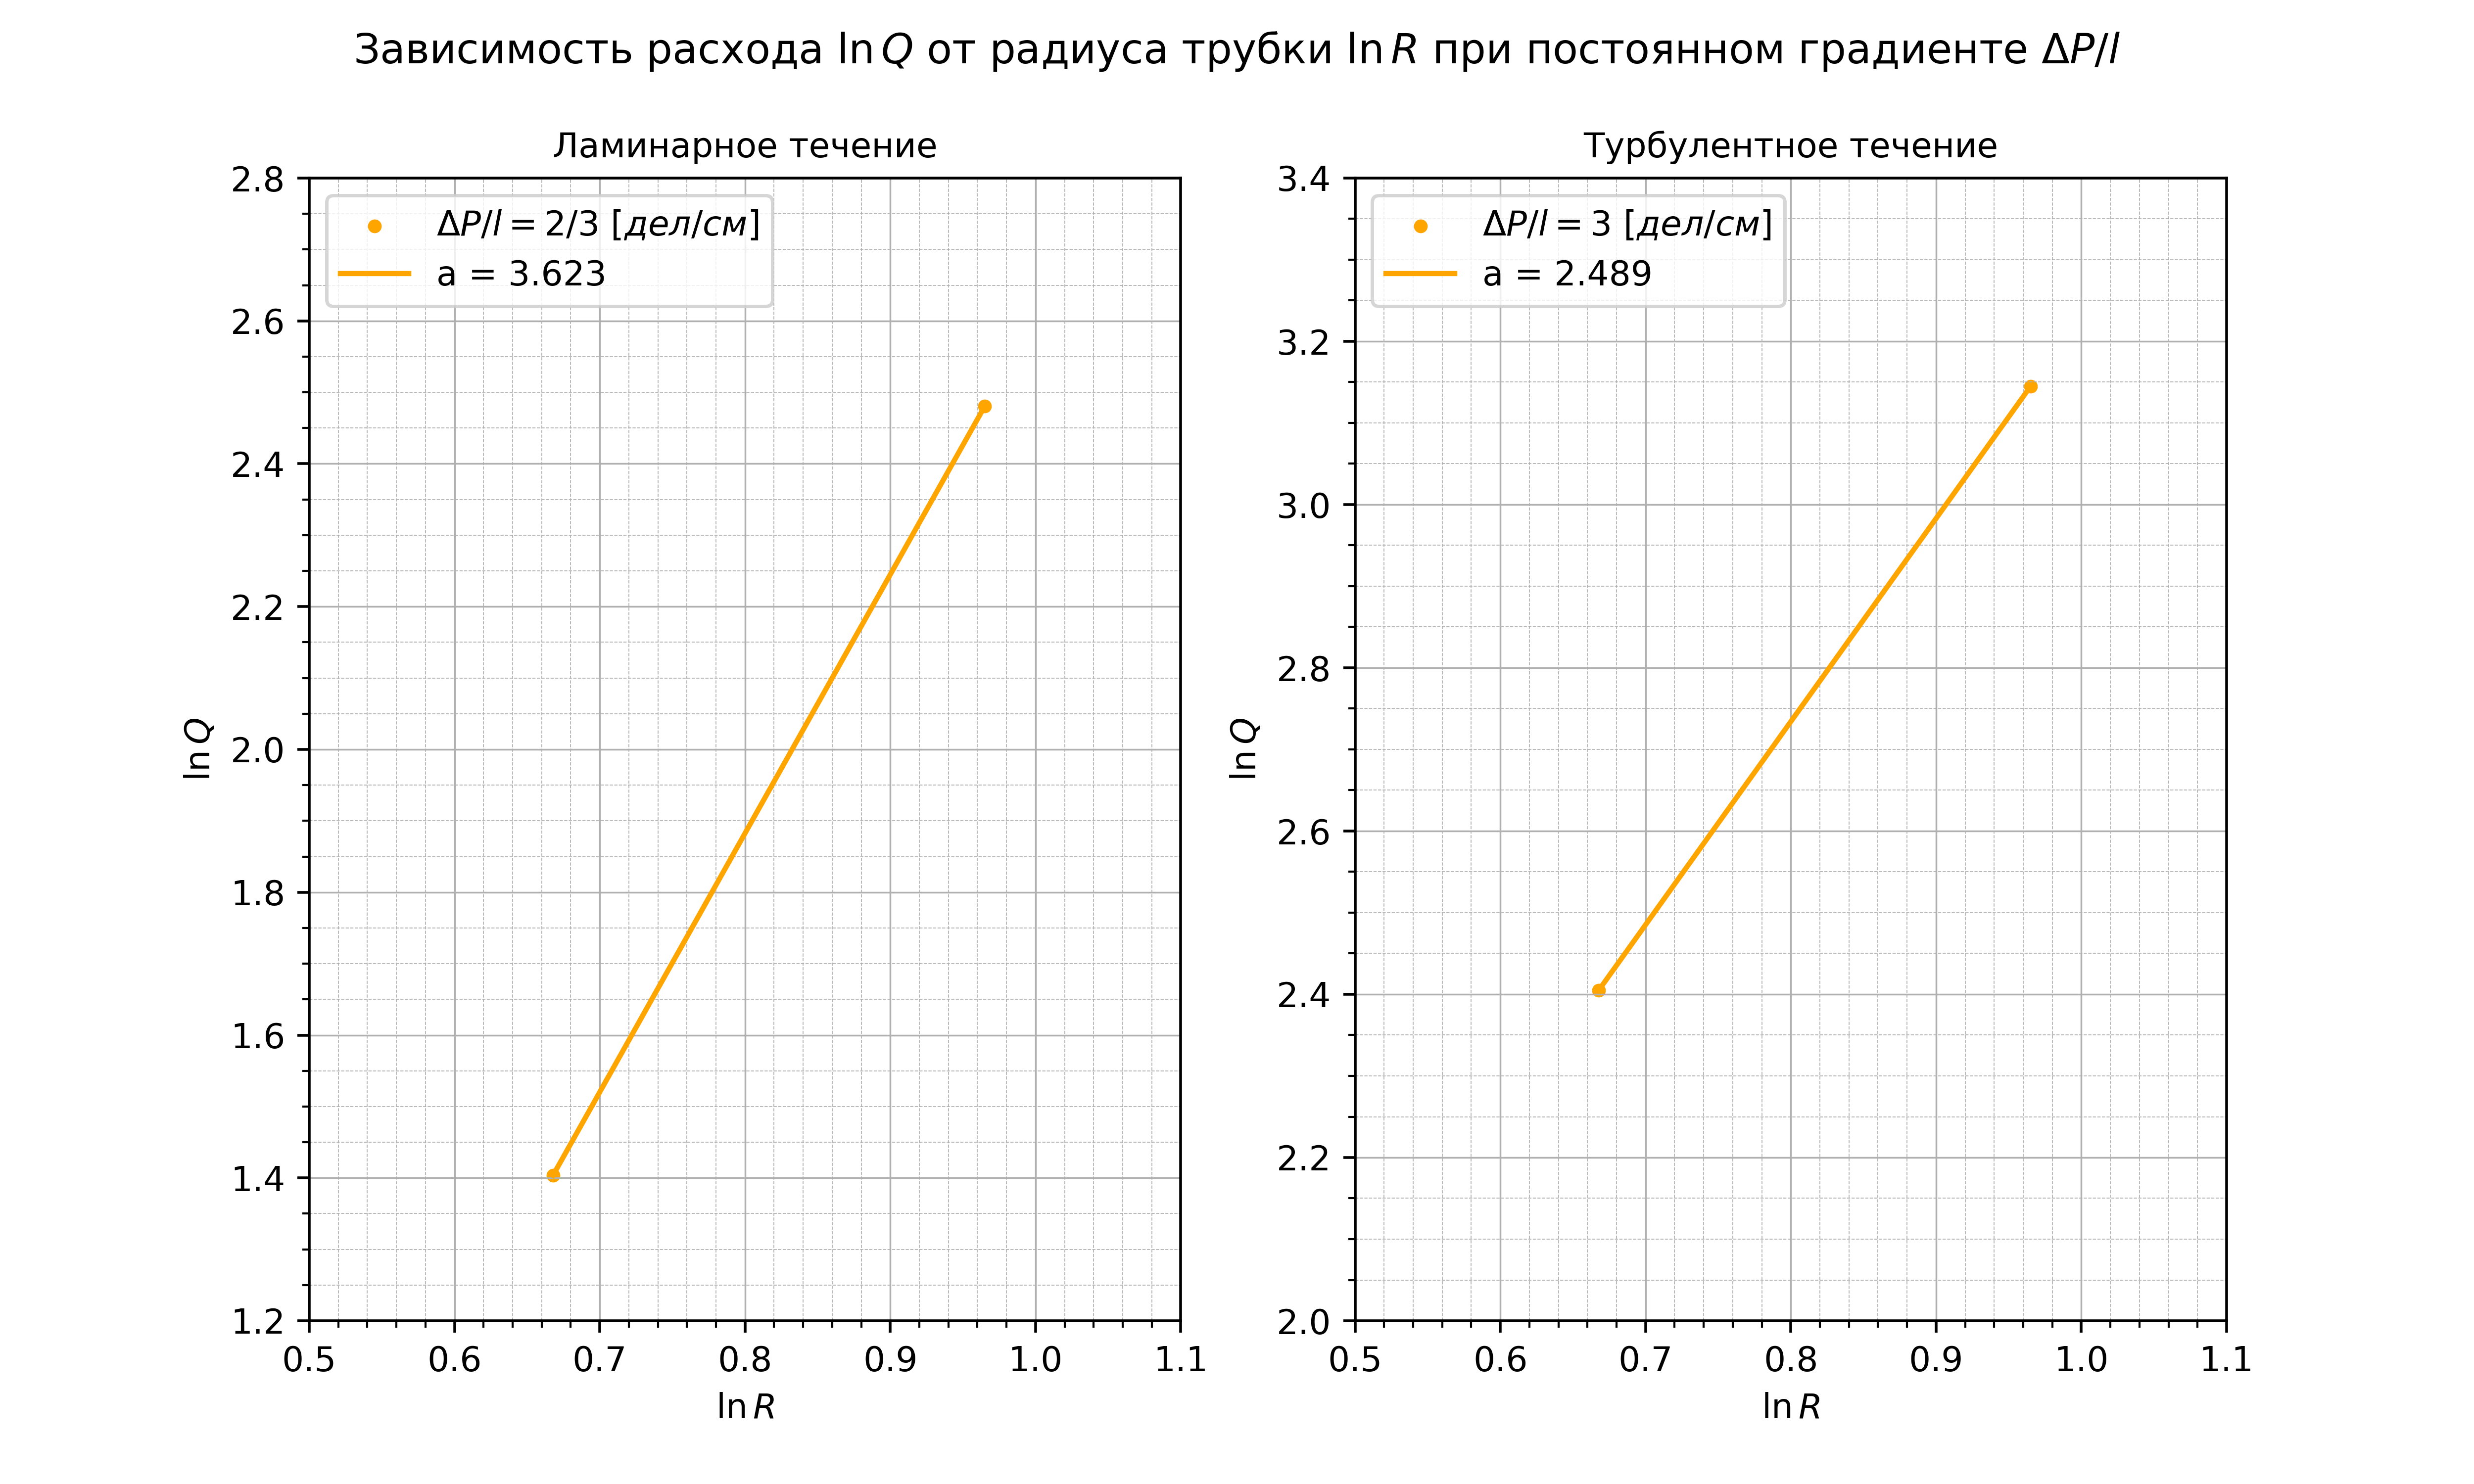
\includegraphics[scale=0.75]{1.3.3_5.png}
\end{flushleft}
\caption{}
\label{ris10}
\end{figure}
Полученные значение показателя степени $\beta$ зависимости $Q \propto R^{\beta}$: при ламинарном течении $\beta \approx 3,6$, при турбулентном течении $\beta \approx 2,5$.

\section{Обсуждение результатов и выводы}
\par В работе изучалась зависимость расхода воздуха от перепада давления на заданном участке трубки. По полученным данным вычислялись вязкость воздуха, критическое число Рейнольдса, а также распределение давления по трубе $P(x)$. Полученные значения вязкости воздуха $\eta$ и критического числа Рейнольдса $Re_{кр}$ представленны в таблице \ref{tab9}. Использованный в работе метод измерений позволяет достичь точности результатов в 5\%. Основной вклад в погрешность результатов вносит погрешность определения времени протекания воздуха, вызванная конечностью времени реакции человека. Полученные результаты соответсвуют табличным значениям вязкости ($18,1 \cdot 10^{-6}~Па \cdot c$) и числа Рейнольдса ($1000$). Полученные результаты распределения давления соотвествуют расчётным.
\begin{table}[h!]
\begin{center}
\begin{tabular}{|c|c|c|}
\hline
      & $\eta, Па \cdot с$           & $Re_{кр}$  \\ \hline
$d_1$ & $19,82\pm0,81 \cdot 10^{-6}$ & $919\pm39$ \\ \hline
$d_2$ & $19,01\pm1,01 \cdot 10^{-6}$ & $844\pm47$ \\ \hline
\end{tabular}
\caption{Полученные результаты}
\label{tab9}
\end{center}
\end{table}
\par Также в данной работе проверялся тот факт, что расход в ламинарном режиме пропорционален четвёртой степени радиуса трубы $Q \propto R^{4}$, а в турбулентном режиме -- $Q \propto R^{2,5}$ (закон Пуазейля). Полученные значения показателя степени -- $3,6$ в ламинарном режиме и $2,5$ в турбулентном -- соответсвуют теоретической модели.

\end{document}
